\chapter{Revisão Bibliográfica}

\section{Fundamentação teórica}

\subsection{Direcionamento por coordenadas geográficas}

Coordenadas geográficas são definidas por dois valores, latitude e longitude, associadas a coordenadas esféricas referenciadas a partir do centro da terra, assumindo o raio da coordenada como o raio médio da superfície do planeta, cerca de $R_\text{Terra} = \SI{6371E3}{\metre}$ \cite{palomaguitarrara, chrisveness}.
A latitude equivale à componente polar $\phi$ centralizada na linha do equador, enquanto a longitude equivale à componente $\theta$ centralizado do meridiano de Greenwich \cite{palomaguitarrara, henriquefleming2003}.

Conhecendo as coordenadas de dois pontos distintos A e B, é possível determinar seu ângulo de \textit{bearing} \ac{betab} relativo, referente ao norte, ou seja, o ângulo da direção a se seguir partindo do ponto A para chegar ao ponto B, a partir da direção norte no ponto de origem A \cite{henriquefleming2003}.

Sendo \textcolor{Green}{\ac{Ag}} e \textcolor{Blue}{\ac{Bg}} duas coordenadas geográficas, \textcolor{Green}{\ac{phiA}} e \textcolor{Blue}{\ac{phiB}} suas respectivas latitudes,  \textcolor{Green}{\ac{thetaA}} e \textcolor{Blue}{\ac{thetaB}} suas respectivas longitudes, conforme ilustrado na \autoref{fig:globo}.

\begin{figure}[htbp]
    \centering
    \caption{Representação geométrica de distância e ângulo em relação ao norte entre coordenadas geográficas \textcolor{Green}{\ac{Ag}} e \textcolor{Blue}{\ac{Bg}}.}
    \begin{tikzpicture}[scale=1,tdplot_main_coords,every node/.style={font = {\footnotesize\bfseries}}]
% https://latex.org/forum/viewtopic.php?t=25316

\def\rvec{3.5}

\def\phivecA{30}
\def\thetavecA{75}

\def\phivecB{45}
\def\thetavecB{15}

\def\auxOpacity{0.75}

\pgfmathsetmacro{\ax}{\rvec*sin(\phivecA)*cos(\thetavecA)}
\pgfmathsetmacro{\ay}{\rvec*sin(\phivecA)*sin(\thetavecA)}
\pgfmathsetmacro{\az}{\rvec*cos(\phivecA)}

\pgfmathsetmacro{\bx}{\rvec*sin(\phivecB)*cos(\thetavecB)}
\pgfmathsetmacro{\by}{\rvec*sin(\phivecB)*sin(\thetavecB)}
\pgfmathsetmacro{\bz}{\rvec*cos(\phivecB)}


\shadedraw[tdplot_screen_coords, ball color = white, opacity=0.25] (0,0) circle (\rvec);

%-----------------------
\coordinate (O) at (0,0,0);

\tdplotsetcoord{A}{\rvec}{\phivecA}{\thetavecA}

\tdplotsetcoord{B}{\rvec}{\phivecB}{\thetavecB}

\tdplotsetcoord{N}{\rvec}{0}{90}

%draw the main coordinate system axes
\draw[thick,-latex] (O) -- (1.35*\rvec,0,0) node[anchor=north east]{$x$};
\draw[thick,-latex] (O) -- (0,1.35*\rvec,0) node[anchor=north west]{$y$};
\draw[thick,-latex] (O) -- (0,0,1.35*\rvec) node[anchor=south]{$z$};

\draw[thick,-latex,opacity=0] (O) -- (-1.35*\rvec,0,0) node[anchor=south west]{$x$};
\draw[thick,-latex,opacity=0] (O) -- (0,-1.35*\rvec,0) node[anchor=south east]{$y$};
\draw[thick,-latex,opacity=0] (O) -- (0,0,-1.35*\rvec) node[anchor=north]{$z$};


\draw[-latex,very thick,opacity=\auxOpacity, color=Green] (O) -- (A) node[anchor=south west, opacity=1] {\ac{Ag}};
\draw[-latex,very thick,opacity=\auxOpacity, color=Blue] (O) -- (B) node[anchor=south east, opacity=1] {\ac{Bg}};
\draw[very thick,color=Black] (N) node[anchor=west] {$\mathbf{N}$};


\draw[dashed, opacity=0.15] (\rvec,0,0) arc (0:360:\rvec);
\draw[thin] (\rvec,0,0) arc (0:135:\rvec);
\draw[thin] (\rvec,0,0) arc (0:-45:\rvec);

\draw[dashed, color=Green, opacity=\auxOpacity] (O) -- (Axy) -- (A);
\draw[dashed, color=Blue, opacity=\auxOpacity] (O) -- (Bxy) -- (B);

\draw[dotted, color=Green, opacity=\auxOpacity] (Ax) -- (Axy);
\draw[dotted, color=Green, opacity=\auxOpacity] (Ay) -- (Axy);

\draw[dotted, color=Blue, opacity=\auxOpacity] (Bx) -- (Bxy);
\draw[dotted, color=Blue, opacity=\auxOpacity] (By) -- (Bxy);

% \pause


\tdplotdrawarc[color=Green, opacity=\auxOpacity]{(O)}{0.75*\rvec}{0}{\thetavecA}{anchor=north}{\ac{thetaA}}

\tdplotdrawarc[color=Blue, opacity=\auxOpacity]{(O)}{0.5*\rvec}{0}{\thetavecB}{anchor=north east}{\ac{thetaB}}

% \pause


\tdplotsetthetaplanecoords{\thetavecA}
\tdplotdrawarc[color=Green, opacity=\auxOpacity, tdplot_rotated_coords]{(O)}{0.75*\rvec}{90}{\phivecA}{anchor=west}{\ac{phiA}}

\tdplotsetthetaplanecoords{\thetavecB}
\tdplotdrawarc[color=Blue, opacity=\auxOpacity, tdplot_rotated_coords]{(O)}{0.5*\rvec}{90}{\phivecB}{anchor=east}{\ac{phiB}}

% \pause

\tdplotsetthetaplanecoords{\thetavecB}
\draw[dashed, Blue, opacity=0.15, tdplot_rotated_coords] (\rvec,0,0) arc (180:-40:-\rvec);
\draw[thin, Blue, opacity=0.25, tdplot_rotated_coords] (\rvec,0,0) arc (0:140:\rvec);
\draw[thin, Blue, opacity=0.25, tdplot_rotated_coords] (\rvec,0,0) arc (360:320:\rvec);
\draw[very thick, color=Blue, tdplot_rotated_coords] (\rvec,0,0) arc (0:\phivecB:\rvec);

\tdplotsetthetaplanecoords{\thetavecA}
\draw[dashed, Green, opacity=0.15, tdplot_rotated_coords] (\rvec,0,0) arc (180:-40:-\rvec);
\draw[thin, Green, opacity=0.25, tdplot_rotated_coords] (\rvec,0,0) arc (0:140:\rvec);
\draw[thin, Green, opacity=0.25, tdplot_rotated_coords] (\rvec,0,0) arc (360:320:\rvec);
\draw[very thick, color=Green, tdplot_rotated_coords] (\rvec,0,0) arc (0:\phivecA:\rvec);


\drawArc{\ax}{\ay}{\az}{\bx}{\by}{\bz}{\rvec}{anchor=south}{\ac{dAB}}

\tdplotsetrotatedcoords{\phivecA}{\thetavecA}{0}

\def\centerarc[#1](#2)(#3:#4:#5)% Syntax: [draw options] (center) (initial angle:final angle:radius)
    { \draw[#1] ($(#2)+({#5*cos(#3)},{#5*sin(#3)})$) arc (#3:#4:#5) node[midway,anchor=south east] {\ac{betab}}; }

\centerarc[Red, tdplot_rotated_coords](A)(292:214:0.4)

\end{tikzpicture}
    % 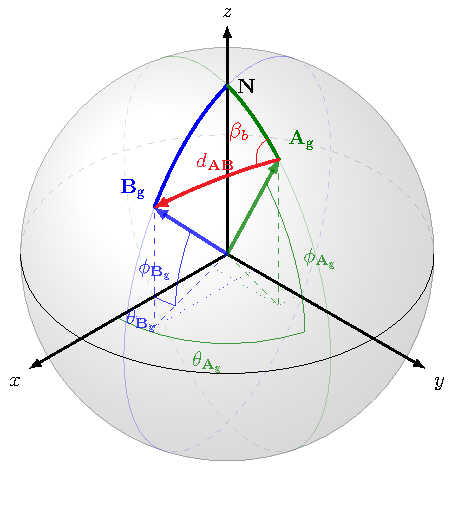
\includegraphics{../pictures/globo.pdf}
    \caption*{Fonte: Autor.}
    \label{fig:globo}
\end{figure}

Calculam-se \ac{Deltaphi} e \ac{Deltatheta}.

    \begin{equation}
        \ac{Deltaphi} = \textcolor{Blue}{\ac{phiB}} - \textcolor{Green}{\ac{phiA}}
    \end{equation}
    \begin{equation}
        \ac{Deltatheta} = \textcolor{Blue}{\ac{thetaB}} - \textcolor{Green}{\ac{thetaA}}
    \end{equation}

Através da lei dos haversines é possível obter a distância mínima $d$ entre as coordenadas, sobre a superfície, e também o ângulo de \textit{Bearing} \textcolor{Red}{\ac{betab}} formado no vértice \textcolor{Green}{\ac{Ag}} do triângulo esférico $\mathbf{N}\textcolor{Green}{\ac{Ag}}\textcolor{Blue}{\ac{Bg}}$ \cite{chrisveness}.
Para o cálculo de distância, os ângulos devem ser tratados em radianos.

\begin{equation}
    X = \cos\left(\textcolor{Blue}{\ac{thetaB}}\right)\cdot \sin\left(\ac{Deltaphi}\right)
\end{equation}
\begin{equation}
    Y = \cos\left(\textcolor{Green}{\ac{thetaA}}\right)\cdot\sin\left(\textcolor{Blue}{\ac{thetaB}}\right) - \sin\left(\textcolor{Green}{\ac{thetaA}}\right) \cdot \cos\left(\textcolor{Green}{\ac{thetaB}}\right) \cdot \cos\left(\ac{Deltaphi}\right)
\end{equation}
\begin{equation}
    Z = \sin^2\left(\frac{\ac{Deltatheta}}{2}\right) + \cos\left(\textcolor{Blue}{\ac{thetaB}}\right) \cdot \cos\left(\textcolor{Green}{\ac{thetaA}}\right) \cdot \sin^2\left(\frac{\ac{Deltaphi}}{2}\right)
\end{equation}
\begin{equation}
    \textcolor{Red}{\ac{betab}} = \arctan\left(\frac{X}{Y}\right) - \frac{\pi}{2}
\end{equation}
\begin{equation}
    \textcolor{Red}{\ac{dAB}} = R_\text{Terra} \cdot 2 \cdot \arctan\left(\frac{\sqrt{Z}}{\sqrt{1-Z}}\right)
\end{equation}

O ângulo \textcolor{Red}{\ac{betab}} calculado aqui é referente à direção cardeal Norte, assim, uma equipe de busca equipada com uma bússola simples seria capaz de seguir a direção correta.
A \autoref{fig:bearing} apresenta a aplicação desenvolvida por \citeauthor{chrisveness}, capaz de calcular o ângulo de \textit{Bearing} entre duas coordenadas, note que, neste caso, o ângulo referido é relacionado à direção cardial Leste \cite{chrisveness}.

\begin{figure}[htbp]
    \centering
    \caption{Cálculo do ângulo de \textit{Bearing} \textcolor{Red}{\ac{betab}} entre as coordenadas dos Campi Santo André e São Bernardo do Campo da UFABC.}
    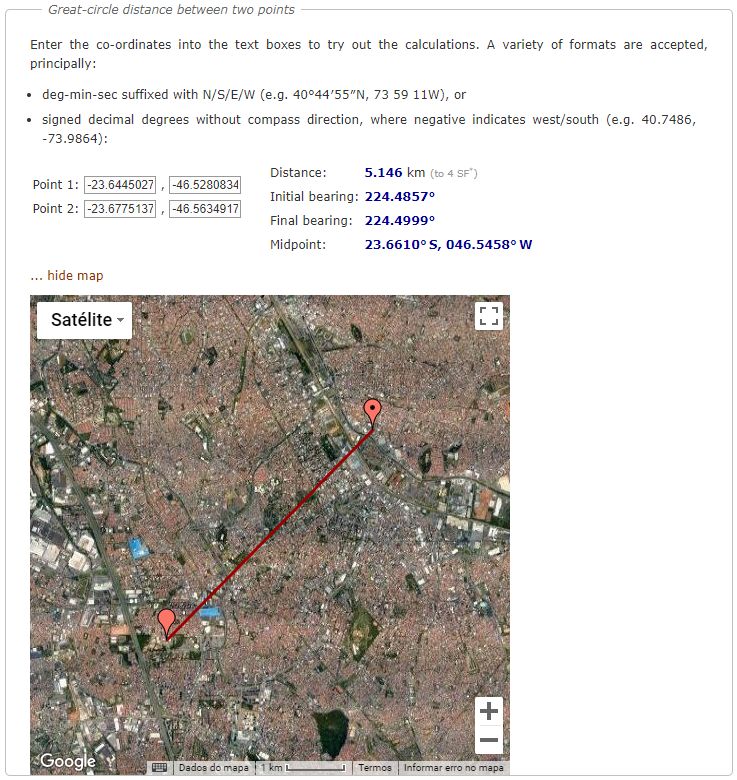
\includegraphics[width=0.7\textwidth]{../pictures/bearing.png}
    \caption*{Fonte: \citeauthor{chrisveness} 2019 \cite{chrisveness}}
    \label{fig:bearing}
\end{figure}

% \pagebreak
% \subsection{Estimar \acs{AoA} utilizando matriz de antenas}

Analisando a defasagem de sinal \ac{RF} em um conjunto de antenas, é possível estimar seu \acf{AoA}, essa técnica pode ser utilizada para determinar a direção do emissor em relação à matriz de antenas utilizada.
Baseando-se em dados como a distância entre as antenas, o comprimento de onda $\lambda$ do sinal e a velocidade da luz no meio, usualmente tomada como $c = \SI{299792458,6 \pm 0,3}{\metre\per\second}$ no ar \cite{jennings1987continuity, bensky2016wireless, horst2021localization}.
A \autoref{eq:wavelength} apresenta a relação do comprimento de onda $\lambda$ com a frequência $f$, com a frequência angular $\omega$ e a velocidade da luz $c$.

\begin{equation}\label{eq:wavelength}
    \lambda = \frac{c}{f} = \frac{2\pi \cdot c}{\omega}
\end{equation}

Se um emissor estiver distante o bastante, é possível considerar que sua frente de onda tem um comportamento planar, essa característica simplifica as operações envolvidas.
A distância de Fraunhofer ($d_F$) é a mínima para essa condição, que define o início da região de \textit{far-field}, conforme apresentado na \autoref{eq:fraunhofer}, onde $D$ é a maior dimensão da antena \cite{balanis2016antenna}.
Tomando $D = 2  \lambda$, para uma antena de dipolo, obtém-se $d_F = 8 \lambda$.
A \autoref{fig:plana_0} ilustra o comportamento planar de uma frente de onda além de $d_F$.

\begin{equation}\label{eq:fraunhofer}
    d_F = \frac{2 \cdot D^2}{\lambda} \quad \Rightarrow \quad d_F = \frac{2 \cdot \left(2 \cdot \lambda \right)^2}{\lambda} = 8 \lambda
\end{equation}

\begin{figure}[htpb]
    \centering
    \caption{Característica de frente de onda a cada $\lambda$ a partir da antena.}
        % \resizebox{\textwidth}{!}{%
    \begin{circuitikz}[american, voltage shift=0.5, line width=0.5]

        \def\wavelength{0.5}
        \def\d{0.5*\wavelength}

        \def\closeRange{1}
        \def\farRange{\closeRange+30}

        \coordinate (O) at (0,0);
        \coordinate (antenna) at (-\closeRange,0);
        % \draw [help lines, dashed] (-5,-3) grid (5,3); % desenha grid
        % \draw [red] (O) node[draw,cross out] {}; % marca pont(0,0)

        \draw[thick]
            (antenna) node[dinantenna, scale=0.75]{}
        ;

        % \draw (\closeRange-0.5,-4) rectangle (\farRange+0.1,4);
        \clip (-0.75,-1.5) rectangle (12.1,1.5);
        \foreach \x [evaluate={\z=int((\x+\closeRange));}] in {0,...,30} {
            \draw [gray, thin, opacity=0.5] (antenna) circle (\z*\wavelength);
            \draw [black]
            (antenna) ++ (\z*\wavelength,0)
            node[anchor=south, font = {\footnotesize\bfseries}, rotate=-90,scale=0.75]{$\z\lambda$}
            ++(0, -4)
            -- ++(0,8);
        }

        \draw [Red, thick] (antenna) ++ (8*\wavelength,-4) -- ++(0,8);

        % \foreach \x in {0,60,...,300} {
        %     \draw[thick] (\x:1 cm) -- (\x + 60:1 cm);

        %     \draw (\x + 30:1.732 cm) node[Gray, circ]{};
        %     \draw[Gray, dashed] (\x:1 cm) -- ++(\x: 0.9cm);
        %     \draw[Gray, dotted]
        %     %     % (\x:1 cm) arc (\x+240:\x+180:1cm)
        %         (\x:1 cm) arc [start angle=\x+120, delta angle=110, radius=1cm]
        %         (\x:1 cm) arc [start angle=\x+120, delta angle=-50, radius=1cm]
        %     ;
        % }

        % \draw (0,0) node [circ] {} node [below left,font={\scriptsize\bfseries}] {BS};
        % \draw[thick, densely dotted] (0,0) circle (1cm);

        % \draw[-latex] (0,0) -- (0:1cm) node[midway, below] {$R_c$};
        % \draw[-latex] (0,0) -- (90:0.866cm) node[midway, left] {$R$};

    \end{circuitikz}
  % }

    % 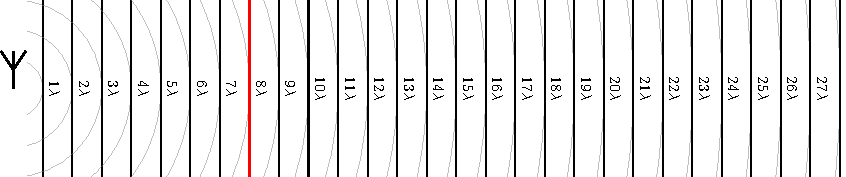
\includegraphics{../pictures/plana_0.pdf}
    \caption*{Fonte: Autor.}
    \label{fig:plana_0}
\end{figure}

Tomando agora um par de antenas separadas por uma distância fixa $d$, torna-se viável fazer a análise trigonométrica entre as antenas e a frente de onda que chega, onde essa distância $d$ será a hipotenusa do triângulo.
A \autoref{fig:AoA} apresenta a disposição das antenas em dois casos de chegada de sinal \ac{RF}.
Para realizar a análise, é necessário conhecer uma segunda dimensão do triângulo retângulo envolvido, esta é obtida analisando a defasagem entre o sinal das antenas, conforme apresentado na \autoref{eq:defasagem}.

\begin{equation}\label{eq:defasagem}
    d \cdot \sin\left(\beta\right) = \lambda \cdot \frac{\Delta\Phi}{2 \pi} \quad \Rightarrow \quad \beta = \arcsin \left(\frac{\lambda}{d} \cdot \frac{\Delta\Phi}{2 \pi}\right)
\end{equation}

É importante ressaltar que um sistemas com um único par de antenas não é capaz de determinar completamente o \ac{AoA}, já que o valor calculado de $\beta$ é igual para casos simétricos, a relação é apresentada nas Figuras \ref{fig:AoA:1} e \ref{fig:AoA:2}.
Existem ainda dois casos notáveis, onde o sinal chega alinhado com a linha das com as antenas ou perpendicular a ela, apresentados respectivamente nas Figuras \ref{fig:AoA:3} e \ref{fig:AoA:4}.

\begin{figure}
    \caption{\ac{AoA} com par de antenas em diversas direções equivalentes.}
    \label{fig:AoA}

    \hfill
    \begin{subfigure}[b]{0.45\textwidth}
        \centering
        \caption{$\beta=\SI{60}{\degree}$}
        % \resizebox{!}{0.7\textheight}{%
\begin{circuitikz}[american, voltage shift=0.5, line width=0.5, every node/.style={font = {\footnotesize\bfseries}}]

    \def\wavelength{3.5}
    \pgfmathsetmacro\d{0.5*\wavelength}

    \def\antennaAngle{20}
    \pgfmathsetmacro\signalAngle{\antennaAngle+40}

    \def\closeRange{9}
    \def\farRange{\closeRange+13}

	\def\NAntennas{3}
	\pgfmathsetmacro\AngleAntennas{360/\NAntennas}
	\def\ShiftAngleAntennas{-90}

	\pgfmathsetmacro\RhoAntennas{\d/(2*sin(180/\NAntennas))}

    \def\centerarc(#1)(#2:#3:#4)% Syntax: [draw options] (center) (initial angle:final angle:radius)
    { ($(#1)+({#4*cos(#2)},{#4*sin(#2)})$) arc (#2:#3:#4) }

    \def\coordref[#1](#2){%

        \coordinate(sysref) at (#2);

        \draw[#1, -latex] (sysref) ++(-0.4,-0.3) -- ++(0.9,0) node[midway, below]{$x$};
        \draw[#1, -latex] (sysref) ++(-0.3,-0.4) -- ++(0,0.9) node[midway, left]{$y$};
        \draw[#1, -latex] \centerarc(sysref)(-90:180:0.25);
        \draw[#1] (sysref) node{$+$}
    }

    \coordinate (bottomleft) at (-3.5,-1);
    \coordinate (topright) at (3.5,5);


    % \draw[Red,dashed] (bottomleft) rectangle (topright);
    \clip (bottomleft) rectangle (topright);

    \coordinate (O) at (0,0);
    \coordinate (sourceAntenna) at (\signalAngle:\closeRange*\wavelength);
    % \draw [help lines, dashed] (bottomleft) grid (topright); % desenha grid
    % \draw [red] (O) node[draw,cross out] {}; % marca pont(0,0)

    % Circulo de antenas
	% \draw[densely dotted, opacity=0.25] (O) ++(90:\RhoAntennas) circle (\RhoAntennas);

    % Linhas do sinal de fundo
    \foreach \x [evaluate={\y=int((\x+\closeRange));\z=int((\x+\closeRange));}] in {-3,...,3} {
        \draw [black!75, very thin]
        (sourceAntenna) ++ (\signalAngle:-\z*\wavelength)
            % node[anchor=west, font = {\footnotesize\bfseries}]{$\y\lambda$}
        ($(sourceAntenna) + (\signalAngle:-\z*\wavelength) + ({10*cos(\signalAngle+90)},{10*sin(\signalAngle+90)})$)
            --
        ($(sourceAntenna) + (\signalAngle:-\z*\wavelength) - ({10*cos(\signalAngle+90)},{10*sin(\signalAngle+90)})$)
        % \draw [gray, thin] (sourceAntenna) circle (\z)
        ;
    }

    % Antenas
    \draw[thick, cmyk_R] (O) node[dinantenna] (A00) {} ;
    % \draw[thick, cmyk_G, opacity=0.75] (O) ++(60:\d) node[dinantenna] (A0d) {} node [below] {$A_{k+2}$};
    \draw[thick, cmyk_B] (O) ++(\antennaAngle:\d) node[dinantenna] (Ad0) {} ;

    \draw[very thin, Black!50, -latex] % Desenha eixo X
        (-3,0) -- (3,0) node[below left] {$x$}
    ;

    % Ângulo alpha entre antenas
    \draw[thin, cmyk_M]
        \centerarc(O)(0:\antennaAngle:0.3)
        node [above, inner sep=3pt] {$\alpha$}
    ;


    % Desenha senoide de fundo
    \draw[Goldenrod, domain=-8:8, samples=100]
        (A00) ++(\signalAngle+90:0.5*\wavelength) coordinate(signalAux)
        plot[shift={(signalAux)}, rotate=\signalAngle]({\x},{cos(\x * pi * 2 / \wavelength r)})
    ;

    % Direção do sinal
    \draw[very thick, dashed, -latex, Goldenrod]
        % (A00) ++(1.5*\d,0) ++ (\signalAngle:-0.5*\d) -- coordinate(angleArrow) ++(\signalAngle:\d)
        (A00) ++(-2,0) ++ (\signalAngle:-0.25*\d) -- coordinate(angleArrow) ++ (\signalAngle:0.5*\d) --++(\signalAngle:0.25*\d)
    ;
    % Angulo Theta do sinal
    \draw[thin]
        (angleArrow) ++ (0.4, 0) node [below,inner sep=2pt] {$\theta_\text{\ac{AoA}}$}
        \centerarc(angleArrow)(0:\signalAngle:0.4)
    ;

    % Triangulo retângulo + quadradinho
    \draw[Black]

        (A00) --++($({\signalAngle-90}:{\d*sin(\signalAngle-\antennaAngle)})$) coordinate (pontoTriangulo) -- (Ad0) -- (A00)

        (pontoTriangulo)
          ++(\signalAngle:0.125)
        --++(\signalAngle+90:0.125)
        --++(\signalAngle+180:0.125)
    ;

    % Arco do angulo beta
    \draw[thin, Purple]
        (Ad0) ++ (180+\antennaAngle:0.4) node[above, inner sep=3pt] {$\beta$}
        \centerarc(Ad0)(180+\antennaAngle:180+\signalAngle:0.4)
    ;

    % Distânci d entre antenas
    \draw[latex-latex]
        ($(A00)+(0,1)$) -- ($(Ad0)+(0,1)$) node [midway, fill=white, circle, inner sep=1pt] {$d$}
    ;

    \newcommand\CircleRadius{3cm}
    %   \draw (0,0) circle (\CircleRadius);
    % special method of noting the position of a point
    \coordinate (P) at (50:\CircleRadius);

\end{circuitikz}
% }


        % 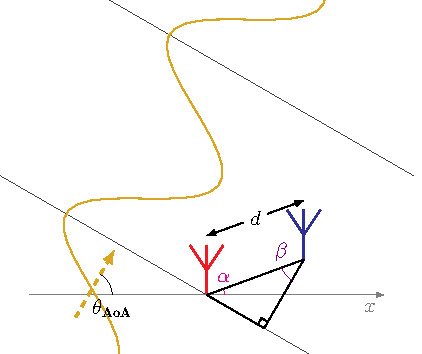
\includegraphics{../pictures/AoA_1.pdf}
        \label{fig:AoA:1}
    \end{subfigure}
    \hfill
    \begin{subfigure}[b]{0.45\textwidth}
        \centering
        \caption{$\beta=\SI{60}{\degree}$}
            % \resizebox{!}{0.7\textheight}{%
    \begin{circuitikz}[american, voltage shift=0.5, line width=0.5,every node/.style={font = {\footnotesize\bfseries}}]

        \def\wavelength{3.5}
        \def\d{0.5*\wavelength}

        \def\antennaAngle{210}

        \def\closeRange{9}
        \def\farRange{\closeRange+13}

        \def\centerarc[#1](#2)(#3:#4:#5)% Syntax: [draw options] (center) (initial angle:final angle:radius)
        { \draw[#1] ($(#2)+({#5*cos(#3)},{#5*sin(#3)})$) arc (#3:#4:#5) node[midway,anchor=west] {$\beta$}; }


        \coordinate (O) at (0,0);
        \coordinate (antenna) at (\antennaAngle:\closeRange*\wavelength);
        % \draw [help lines, dashed] (-5,-3) grid (5,3); % desenha grid
        % \draw [red] (O) node[draw,cross out] {}; % marca pont(0,0) 
        
        % \draw (-6.8,-4) rectangle (6.8,4);
        \clip (-3.5,-3.5) rectangle (3.5,3.5);

        % \draw[thick]
        %     (antenna) node[dinantenna]{}
        % ;
        
        \foreach \x [evaluate={\y=int((\x+\closeRange));\z=int((\x+\closeRange));}] in {-3,...,3} {
            \draw [black, thin] 
            (antenna) ++ (\antennaAngle:-\z*\wavelength)
                % node[anchor=west, font = {\footnotesize\bfseries}]{$\y\lambda$}
            ($(antenna) + (\antennaAngle:-\z*\wavelength) + ({10*cos(\antennaAngle+90)},{10*sin(\antennaAngle+90)})$)
                -- 
            ($(antenna) + (\antennaAngle:-\z*\wavelength) - ({10*cos(\antennaAngle+90)},{10*sin(\antennaAngle+90)})$);
            % \draw [gray, thin] (antenna) circle (\z);
        }
        
        \draw[thick]
            (0,0)  node[Green, dinantenna] (A00) {}
            % (0,\d) node[Blue,  dinantenna] (A0d) {}
            (\d,0) node[Red,   dinantenna] (Ad0) {}
        ;

        \draw[very thick, dashed, -latex]
            (A00) ++(-\d,0) coordinate(aux) ++(\antennaAngle:0.5*\d) -- ++(\antennaAngle:-\d)
        ;

        
        \draw[Goldenrod, domain=-8:8, samples=100] plot[shift={(aux)}, rotate=\antennaAngle]({\x},{sin(\x * pi * 2 / \wavelength r)});
        
        \draw[thin, opacity=0.5]
            (A00) ++ ($({\antennaAngle-90}:{\d*sin(\antennaAngle)})$) -- (Ad0) -- (A00)

            ($({\antennaAngle-90}:{\d*sin(\antennaAngle)})$) 
              ++(\antennaAngle+180:0.125)
            --++(\antennaAngle-90:0.125)
            --++(\antennaAngle:0.125)

            
        ;

        \centerarc[thin, opacity=0.5](A00)(\antennaAngle+90:360:0.4)

        \draw[latex-latex]
            ($(A00)+(0,1)$) -- ($(Ad0)+(0,1)$) node [midway, fill=white] {$d$}
        ;
        


        % \foreach \x in {0,60,...,300} {
        %     \draw[thick] (\x:1 cm) -- (\x + 60:1 cm);
            
        %     \draw (\x + 30:1.732 cm) node[Gray, circ]{};
        %     \draw[Gray, dashed] (\x:1 cm) -- ++(\x: 0.9cm);
        %     \draw[Gray, dotted]
        %     %     % (\x:1 cm) arc (\x+240:\x+180:1cm)
        %         (\x:1 cm) arc [start angle=\x+120, delta angle=110, radius=1cm]
        %         (\x:1 cm) arc [start angle=\x+120, delta angle=-50, radius=1cm]
        %     ;
        % }
    
        % \draw (0,0) node [circ] {} node [below left,font={\scriptsize\bfseries}] {BS};
        % \draw[thick, densely dotted] (0,0) circle (1cm);
        
        % \draw[-latex] (0,0) -- (0:1cm) node[midway, below] {$R_c$};
        % \draw[-latex] (0,0) -- (90:0.866cm) node[midway, left] {$R$};
            
    \end{circuitikz}
  % }


        % 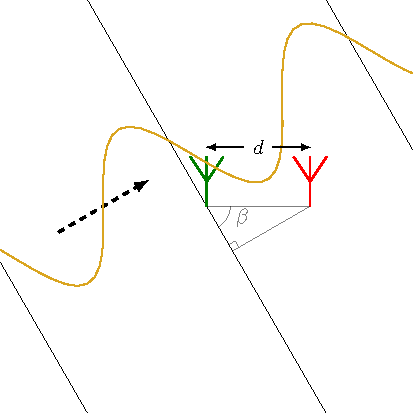
\includegraphics{../pictures/AoA_2.pdf}
        \label{fig:AoA:2}
    \end{subfigure}
    \hfill

    \hfill
    \begin{subfigure}[b]{0.45\textwidth}
        \centering
        \caption{$\beta=\SI{90}{\degree}$}
            % \resizebox{!}{0.7\textheight}{%
    \begin{circuitikz}[american, voltage shift=0.5, line width=0.5,every node/.style={font = {\footnotesize\bfseries}}]

        \def\wavelength{3.5}
        \def\d{0.5*\wavelength}


        \def\antennaAngle{180}
        \def\closeRange{9}
        \def\farRange{\closeRange+13}

        \def\centerarc[#1](#2)(#3:#4:#5)% Syntax: [draw options] (center) (initial angle:final angle:radius)
        { \draw[#1] ($(#2)+({#5*cos(#3)},{#5*sin(#3)})$) arc (#3:#4:#5) node[midway,anchor=west] {$\beta$}; }


        \coordinate (O) at (0,0);
        \coordinate (antenna) at (\antennaAngle:\closeRange*\wavelength);
        % \draw [help lines, dashed] (-5,-3) grid (5,3); % desenha grid
        % \draw [red] (O) node[draw,cross out] {}; % marca pont(0,0) 
        
        % \draw (-6.8,-4) rectangle (6.8,4);
        \clip (-3.5,-3.5) rectangle (3.5,3.5);

        % \draw[thick]
        %     (antenna) node[dinantenna]{}
        % ;
        
        \foreach \x [evaluate={\y=int((\x+\closeRange));\z=int((\x+\closeRange));}] in {-3,...,3} {
            \draw [black, thin] 
            (antenna) ++ (\antennaAngle:-\z*\wavelength)
                % node[anchor=west, font = {\footnotesize\bfseries}]{$\y\lambda$}
            ($(antenna) + (\antennaAngle:-\z*\wavelength) + ({10*cos(\antennaAngle+90)},{10*sin(\antennaAngle+90)})$)
                -- 
            ($(antenna) + (\antennaAngle:-\z*\wavelength) - ({10*cos(\antennaAngle+90)},{10*sin(\antennaAngle+90)})$);
            % \draw [gray, thin] (antenna) circle (\z);
        }
        
        \draw[thick]
            (0,0)  node[Green, dinantenna] (A00) {}
            % (0,\d) node[Blue,  dinantenna] (A0d) {}
            (\d,0) node[Red,   dinantenna] (Ad0) {}
        ;

        \draw[very thick, dashed, -latex]
            (A00) ++(-\d,0) coordinate(aux) ++(\antennaAngle:0.5*\d) -- ++(\antennaAngle:-\d)
        ;

        
        \draw[Goldenrod, domain=-8:8, samples=100] plot[shift={(aux)}, rotate=\antennaAngle]({\x},{cos(\x * pi * 2 / \wavelength r)});
        % \draw[thin, densely dotted]
        %     (A00) ++ ($({\antennaAngle-90}:{\d*sin(\antennaAngle)})$) -- (Ad0) -- (A00)

        %     ($({\antennaAngle-90}:{\d*sin(\antennaAngle)})$) 
        %       ++(\antennaAngle+180:0.25)
        %     --++(\antennaAngle-90:0.25)
        %     --++(\antennaAngle:0.25)

            
        % ;

        % \centerarc[thin, densely dotted](A00)(\antennaAngle+90:360:0.4)

        \draw[latex-latex]
            ($(A00)+(0,1)$) -- ($(Ad0)+(0,1)$) node [midway, fill=white] {$d$}
        ;

        % \draw[color=Blue, samples=100, domain=-4:4, smooth]
        %     (A00)++(-\d,0)
        %     % plot[rotate=\antennaAngle] ({\x},{sin((\x r)*0.31830)})
        % ;


        % \foreach \x in {0,60,...,300} {
        %     \draw[thick] (\x:1 cm) -- (\x + 60:1 cm);
            
        %     \draw (\x + 30:1.732 cm) node[Gray, circ]{};
        %     \draw[Gray, dashed] (\x:1 cm) -- ++(\x: 0.9cm);
        %     \draw[Gray, dotted]
        %     %     % (\x:1 cm) arc (\x+240:\x+180:1cm)
        %         (\x:1 cm) arc [start angle=\x+120, delta angle=110, radius=1cm]
        %         (\x:1 cm) arc [start angle=\x+120, delta angle=-50, radius=1cm]
        %     ;
        % }
    
        % \draw (0,0) node [circ] {} node [below left,font={\scriptsize\bfseries}] {BS};
        % \draw[thick, densely dotted] (0,0) circle (1cm);
        
        % \draw[-latex] (0,0) -- (0:1cm) node[midway, below] {$R_c$};
        % \draw[-latex] (0,0) -- (90:0.866cm) node[midway, left] {$R$};
            
    \end{circuitikz}
  % }


        % 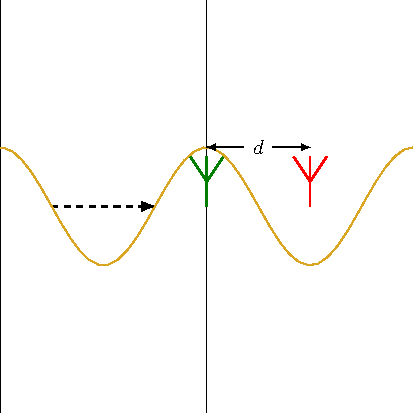
\includegraphics{../pictures/AoA_3.pdf}
        \label{fig:AoA:3}
    \end{subfigure}
    \hfill
    \begin{subfigure}[b]{0.45\textwidth}
        \centering
        \caption{$\beta=\SI{0}{\degree}$}
        % \resizebox{!}{0.7\textheight}{%
\begin{circuitikz}[american, voltage shift=0.5, line width=0.5, every node/.style={font = {\footnotesize\bfseries}}]

    \def\wavelength{3.5}
    \pgfmathsetmacro\d{0.5*\wavelength}

    \def\antennaAngle{20}
    \def\signalAngle{\antennaAngle}

    \def\closeRange{9}
    \def\farRange{\closeRange+13}

	\def\NAntennas{3}
	\pgfmathsetmacro\AngleAntennas{360/\NAntennas}
	\def\ShiftAngleAntennas{-90}

	\pgfmathsetmacro\RhoAntennas{\d/(2*sin(180/\NAntennas))}

    \def\centerarc(#1)(#2:#3:#4)% Syntax: [draw options] (center) (initial angle:final angle:radius)
    { ($(#1)+({#4*cos(#2)},{#4*sin(#2)})$) arc (#2:#3:#4) }

    \def\coordref[#1](#2){%

        \coordinate(sysref) at (#2);

        \draw[#1, -latex] (sysref) ++(-0.4,-0.3) -- ++(0.9,0) node[midway, below]{$x$};
        \draw[#1, -latex] (sysref) ++(-0.3,-0.4) -- ++(0,0.9) node[midway, left]{$y$};
        \draw[#1, -latex] \centerarc(sysref)(-90:180:0.25);
        \draw[#1] (sysref) node{$+$}
    }

    \coordinate (bottomleft) at (-3.5,-1);
    \coordinate (topright) at (3.5,5);


    % \draw[Red,dashed] (bottomleft) rectangle (topright);
    \clip (bottomleft) rectangle (topright);

    \coordinate (O) at (0,0);
    \coordinate (sourceAntenna) at (\signalAngle:\closeRange*\wavelength);
    % \draw [help lines, dashed] (bottomleft) grid (topright); % desenha grid
    % \draw [red] (O) node[draw,cross out] {}; % marca pont(0,0)

    % Circulo de antenas
	% \draw[densely dotted, opacity=0.25] (O) ++(90:\RhoAntennas) circle (\RhoAntennas);

    % Linhas do sinal de fundo
    \foreach \x [evaluate={\y=int((\x+\closeRange));\z=int((\x+\closeRange));}] in {-3,...,3} {
        \draw [black!75, very thin]
        (sourceAntenna) ++ (\signalAngle:-\z*\wavelength)
            % node[anchor=west, font = {\footnotesize\bfseries}]{$\y\lambda$}
        ($(sourceAntenna) + (\signalAngle:-\z*\wavelength) + ({10*cos(\signalAngle+90)},{10*sin(\signalAngle+90)})$)
            --
        ($(sourceAntenna) + (\signalAngle:-\z*\wavelength) - ({10*cos(\signalAngle+90)},{10*sin(\signalAngle+90)})$)
        % \draw [gray, thin] (sourceAntenna) circle (\z)
        ;
    }

    % Antenas
    \draw[thick, cmyk_R] (O) node[dinantenna] (A00) {} ;
    % \draw[thick, cmyk_G, opacity=0.75] (O) ++(60:\d) node[dinantenna] (A0d) {} node [below] {$A_{k+2}$};
    \draw[thick, cmyk_B] (O) ++(\antennaAngle:\d) node[dinantenna] (Ad0) {} ;

    \draw[very thin, Black!50, -latex] % Desenha eixo X
        (-3,0) -- (3,0) node[below left] {$x$}
    ;

    % Ângulo alpha entre antenas
    \draw[thin, cmyk_M]
		(0.3,0) node [below, inner sep=3pt] {$\alpha$}
		\centerarc(O)(0:\antennaAngle:0.3)
    ;


    % Desenha senoide de fundo
    \draw[Goldenrod, domain=-8:8, samples=100]
        (A00) ++(\signalAngle+90:0.75*\wavelength) coordinate(signalAux)
        plot[shift={(signalAux)}, rotate=\signalAngle]({\x},{cos(\x * pi * 2 / \wavelength r)})
    ;

    % Direção do sinal
    \draw[very thick, dashed, -latex, Goldenrod]
        % (A00) ++(1.5*\d,0) ++ (\signalAngle:-0.25*\d) -- coordinate(angleArrow) ++(\signalAngle:0.85*\d)
        (A00) ++(-2,0) ++ (\signalAngle:-0.25*\d) -- coordinate(angleArrow) ++ (\signalAngle:0.5*\d) --++(\signalAngle:0.25*\d)
    ;
    % Angulo Theta do sinal
    \draw[thin]
        (angleArrow) ++ (0.4, 0) node [below,inner sep=2pt] {$\theta_\text{\ac{AoA}}$}
        \centerarc(angleArrow)(0:\signalAngle:0.4)
    ;

    % Triangulo retângulo + quadradinho
    \draw[Black]

    %     % (A00) --++($({\signalAngle-90}:{\d*sin(\signalAngle-\antennaAngle)})$) coordinate (pontoTriangulo) --
		(Ad0) -- (A00)

    %     % (pontoTriangulo)
    %     %   ++(\signalAngle:0.125)
    %     % --++(\signalAngle+90:0.125)
    %     % --++(\signalAngle+180:0.125)
    ;

    % % Arco do angulo beta
    % \draw[thin]
    %     \centerarc(Ad0)(180+\antennaAngle:180+\signalAngle:0.4) node[below, inner sep=3pt] {$\beta$}
    % ;

    % Distânci d entre antenas
    \draw[latex-latex]
        ($(A00)+(0,1)$) -- ($(Ad0)+(0,1)$) node [midway, fill=white, circle, inner sep=1pt] {$d$}
    ;

    \newcommand\CircleRadius{3cm}
    %   \draw (0,0) circle (\CircleRadius);
    % special method of noting the position of a point
    \coordinate (P) at (50:\CircleRadius);

\end{circuitikz}
% }


        % 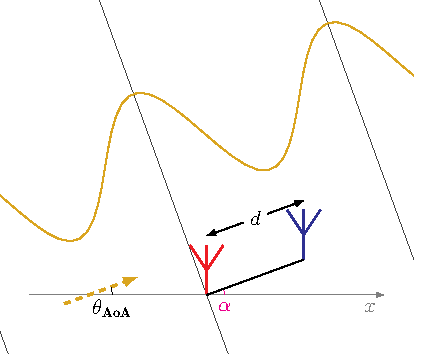
\includegraphics{../pictures/AoA_4.pdf}
        \label{fig:AoA:4}
    \end{subfigure}
    \hfill

    \caption*{Fonte: Autor.}
\end{figure}

A escolha da distância $d$ entre as antenas deve ser feita de forma a otimizar a otimizar a resolução da medida de defasagem, com a maior distância possível, porém é necessário evitar ambiguidades na análise, como o sinal é periódico, o valor se repetirá a cada $\lambda$, e terá valores simétricos quando $d > \sfrac{\lambda}{2}$, ilustrado na \autoref{fig:AoA_d:fail}.
Adota-se então $d=\sfrac{\lambda}{2}$, conforme apresentado na \autoref{fig:AoA_d:ok} \cite{bensky2016wireless, horst2021localization}.

\begin{figure}
    \caption{Diferentes valores para $d$.}
    \label{fig:AoA_d}

    \hfill
    \begin{subfigure}[b]{0.45\textwidth}
        \centering
        \caption{$d > \sfrac{\lambda}{2}$}
            % \resizebox{!}{0.7\textheight}{%
    \begin{circuitikz}[american, voltage shift=0.5, line width=0.5,every node/.style={font = {\footnotesize\bfseries}}]

        \def\wavelength{4}
        \def\d{0.5*\wavelength}


        \def\antennaAngle{120}
        \def\closeRange{9}
        \def\farRange{\closeRange+13}

        \def\centerarc[#1](#2)(#3:#4:#5)% Syntax: [draw options] (center) (initial angle:final angle:radius)
        { \draw[#1] ($(#2)+({#5*cos(#3)},{#5*sin(#3)})$) arc (#3:#4:#5) node[midway,anchor=west] {$\beta$}; }


        \coordinate (O) at (0,0);
        \coordinate (antenna) at (\antennaAngle:\closeRange*\wavelength);
        % \draw [help lines, dashed] (-3,-3) grid (3,3); % desenha grid
        % \draw [red] (O) node[draw,cross out] {}; % marca pont(0,0)

        % \draw (-6.8,-4) rectangle (6.8,4);
        \clip (-1,-1.1) rectangle (5,1.1);


        \draw[thick]
            (0,0)  node[cmyk_B, dinantenna] (A00) {}
            % (0,\d) node[Blue,  dinantenna] (A0d) {}
            (1.2*\d,0) node[cmyk_R,   dinantenna] (Ad0) {}
            (0.8*\d,0) node[cmyk_R,   dinantenna, opacity=0.2] (Ad0_phantom) {}
        ;

        % \draw[Goldenrod, domain=-3:3, samples=100] plot[shift={(-1,-1)}, rotate=30]({\x},{sin(\x * pi * 2 / \wavelength r)});
        \draw[Goldenrod, domain=-3:6, samples=50]
            plot ({\x},{cos(\x * pi * 2 / \wavelength r)})
        ;

        \draw[Black, dashed, domain=-3:6, samples=2]
            plot[Black, thin, dashed, samples=2] (\x,0)
        ;

        \draw [densely dotted, cmyk_R]
            (Ad0_phantom) --
            ++(0,{cos(1.2*\d * pi * 2 / \wavelength r)}) --
            ++({0.4*\d},0) --
            (Ad0)
        ;

    \end{circuitikz}
  % }
        % 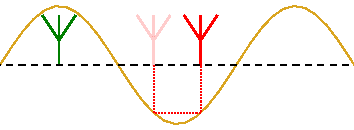
\includegraphics{../pictures/AoA_0_fail.pdf}
        \label{fig:AoA_d:fail}
    \end{subfigure}
    \hfill
    \begin{subfigure}[b]{0.45\textwidth}
        \centering
        \caption{$d = \sfrac{\lambda}{2}$}
            % \resizebox{!}{0.7\textheight}{%
    \begin{circuitikz}[american, voltage shift=0.5, line width=0.5,every node/.style={font = {\footnotesize\bfseries}}]

        \def\wavelength{4}
        \def\d{0.5*\wavelength}


        \def\antennaAngle{120}
        \def\closeRange{9}
        \def\farRange{\closeRange+13}

        \def\centerarc[#1](#2)(#3:#4:#5)% Syntax: [draw options] (center) (initial angle:final angle:radius)
        { \draw[#1] ($(#2)+({#5*cos(#3)},{#5*sin(#3)})$) arc (#3:#4:#5) node[midway,anchor=west] {$\beta$}; }


        \coordinate (O) at (0,0);
        \coordinate (antenna) at (\antennaAngle:\closeRange*\wavelength);
        % \draw [help lines, dashed] (-3,-3) grid (3,3); % desenha grid
        % \draw [red] (O) node[draw,cross out] {}; % marca pont(0,0) 
        
        % \draw (5,1.25) rectangle (-1,-1.1);
        \clip (5,1.25) rectangle (-1,-1.1);

        
        % \draw[Goldenrod, domain=-3:3, samples=100] plot[shift={(-1,-1)}, rotate=30]({\x},{sin(\x * pi * 2 / \wavelength r)});
        \draw[Goldenrod, domain=-3:6, samples=50] 
            plot ({\x},{cos(\x * pi * 2 / \wavelength r)})
        ;
        
        \draw[Black, dashed, domain=-3:6, samples=2] 
            plot[Black, thin, dashed, samples=2] (\x,0)
        ;
        
        
        % \pause
        \draw[thick]
            (0,0)  node[Green, dinantenna] (A00) {}
            % (0,\d) node[Blue,  dinantenna] (A0d) {}
            % (\d,0) node[Red,   dinantenna] (Ad0) {}
        ;
        
        % \pause
        \draw[thick]
            % (0,0)  node[Green, dinantenna] (A00) {}
            % (0,\d) node[Blue,  dinantenna] (A0d) {}
            (\d,0) node[Red,   dinantenna] (Ad0) {}
        ;

        \draw[latex-latex]
            ($(A00)+(0,1.1)$) -- ++(\wavelength,0) node [midway, fill=white] {$\lambda$}
        ;
    % \visible<7->{
        \draw[latex-latex]
            ($(A00)+(0,-0.1)$) -- ++(0.5*\wavelength,0) node [midway, fill=white, fill opacity=0.75, anchor=north] {$d = \sfrac{\lambda}{2}$}
        ;
    % }
            
    \end{circuitikz}
  % }
        % 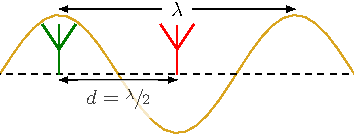
\includegraphics{../pictures/AoA_0.pdf}
        \label{fig:AoA_d:ok}
    \end{subfigure}
    \hfill

    \caption*{Fonte: Autor.}
\end{figure}

Para contornar a ambiguidade gerada pela simetria no sistema, é possível adicionar uma terceira antena, de forma que não esteja alinhada com as duas primeiras.
Um exemplo é apresentado na \autoref{fig:AoA_5}.

\begin{figure}[htbp]
    \centering
    \caption{Possível disposição de matriz de antenas.}
        % \resizebox{!}{0.7\textheight}{%
    \begin{circuitikz}[american, voltage shift=0.5, line width=0.5,every node/.style={font = {\footnotesize\bfseries}}]

        \def\wavelength{4}
        \def\d{0.5*\wavelength}


        \def\antennaAngle{240}
        \def\closeRange{9}
        \def\farRange{\closeRange+13}

        \def\centerarc[#1](#2)(#3:#4:#5)(#6)(#7)% Syntax: [draw options] (center) (initial angle:final angle:radius)
        { \draw[#1] ($(#2)+({#5*cos(#3)},{#5*sin(#3)})$) arc (#3:#4:#5) node[midway,anchor=#7] {#6}; }


        \coordinate (O) at (0,0);
        \coordinate (antenna) at (\antennaAngle:\closeRange*\wavelength);
        % \draw [help lines, dashed] (-5,-3) grid (5,3); % desenha grid
        % \draw [red] (O) node[draw,cross out] {}; % marca pont(0,0)

        % \draw (-6.8,-4) rectangle (6.8,4);
        \clip (-6.8,-4) rectangle (6.8,4);

        % \draw[thick]
        %     (antenna) node[dinantenna]{}
        % ;

        \foreach \x [evaluate={\y=int((\x+\closeRange));\z=int((\x+\closeRange)*\wavelength);}] in {-3,...,3} {
            \draw [black, thin]
            (antenna) ++ (\antennaAngle:-\z)
                % node[anchor=west, font = {\footnotesize\bfseries}]{$\y\lambda$}
            ($(antenna) + (\antennaAngle:-\z) + ({10*cos(\antennaAngle+90)},{10*sin(\antennaAngle+90)})$)
                --
            ($(antenna) + (\antennaAngle:-\z) - ({10*cos(\antennaAngle+90)},{10*sin(\antennaAngle+90)})$);
            % \draw [gray, thin] (antenna) circle (\z);
        }

        \draw[thick]
            (0,0)  node[Green, dinantenna] (A00) {}
            (0,\d) node[Blue,  dinantenna] (A0d) {}
            (\d,0) node[Red,   dinantenna] (Ad0) {}
        ;

        \draw[very thick, dashed, -latex]
            (A00) ++(-\d,0) coordinate(aux) ++(\antennaAngle:0.5*\d) -- ++(\antennaAngle:-\d)
        ;


        % \draw[antena_5_5, domain=-8:8, samples=100] plot[shift={(aux)}, rotate=\antennaAngle]({\x},{sin(\x * pi * 2 / \wavelength r)});

        \draw[thin, Red, opacity=0.5]
            (A00) ++ ($({\antennaAngle-90}:{\d*sin(\antennaAngle)})$) -- (Ad0) -- (A00)

            ($({\antennaAngle-90}:{\d*sin(\antennaAngle)})$)
              ++(\antennaAngle+180:0.25)
            --++(\antennaAngle-90:0.25)
            --++(\antennaAngle:0.25)
        ;


        \centerarc[thin, Red, opacity=0.5](A00)(\antennaAngle+90:360:0.4)($\beta_{0d}$)(north)


        \draw[thin, Blue, opacity=0.5]
            (A00) ++ ($({\antennaAngle+90}:{\d*cos(\antennaAngle)})$) -- (A0d) -- (A00)

            ($({\antennaAngle+90}:{\d*cos(\antennaAngle)})$)
              ++(\antennaAngle+180:0.25)
            --++(\antennaAngle+90:0.25)
            --++(\antennaAngle:0.25)
        ;

        \centerarc[thin, Blue, opacity=0.5](A00)(\antennaAngle-90:90:0.4)($\beta_{d0}$)(north east)

        \draw[latex-latex]
            ($(A00)+(0,1)$) -- ($(Ad0)+(0,1)$) node [midway, fill=white] {$d$}
        ;



        % \foreach \x in {0,60,...,300} {
        %     \draw[thick] (\x:1 cm) -- (\x + 60:1 cm);

        %     \draw (\x + 30:1.732 cm) node[Gray, circ]{};
        %     \draw[Gray, dashed] (\x:1 cm) -- ++(\x: 0.9cm);
        %     \draw[Gray, dotted]
        %     %     % (\x:1 cm) arc (\x+240:\x+180:1cm)
        %         (\x:1 cm) arc [start angle=\x+120, delta angle=110, radius=1cm]
        %         (\x:1 cm) arc [start angle=\x+120, delta angle=-50, radius=1cm]
        %     ;
        % }

        % \draw (0,0) node [circ] {} node [below left,font={\scriptsize\bfseries}] {BS};
        % \draw[thick, densely dotted] (0,0) circle (1cm);

        % \draw[-latex] (0,0) -- (0:1cm) node[midway, below] {$R_c$};
        % \draw[-latex] (0,0) -- (90:0.866cm) node[midway, left] {$R$};

    \end{circuitikz}
  % }


    % 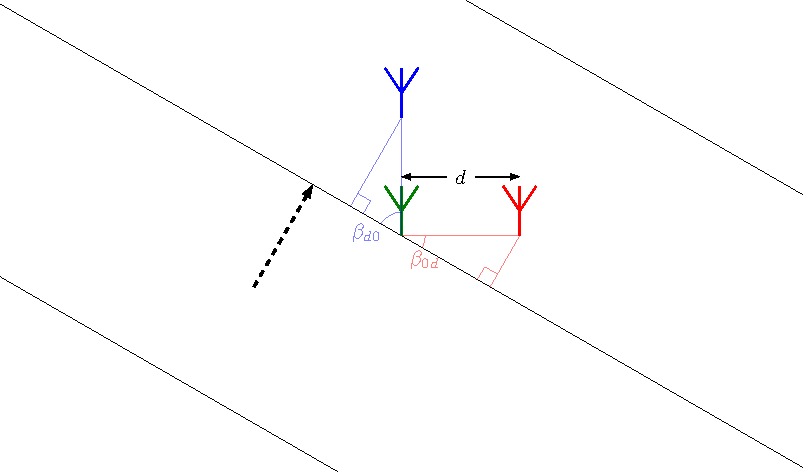
\includegraphics{../pictures/AoA_5.pdf}
    \caption*{Fonte: Autor.}
    \label{fig:AoA_5}
\end{figure}

Para obter o valor de defasagem entre antenas, é interessante representar o sinal recebido como um valor complexo.
Uma forma de obter o valor complexo é realizando a integração de período completo no produto do sinal recebido na antena por uma senoide ou cossenoide de mesma frequência.
Nas Equações \ref{eq:S} e \ref{eq:C}, $S$ e $C$ são respectivamente proporcionais às componentes em fase e em quadratura do sinal $w$ recebido na antena, $k$ é uma função auxiliar que garante frequência correta em todos os operandos.
É válido notar que $w$ e $k$ são funções de várias variáveis.

\begin{equation}\label{eq:S}
    S = \int_0^T w(t) \cdot \sin(k(t)) \partial t
\end{equation}

\begin{equation}\label{eq:C}
    C = \int_0^T w(t) \cdot \cos(k(t)) \partial t
\end{equation}

Finalmente, na \autoref{eq:Z}, $Z$ é o valor complexo associada ao sinal recebido em na antena.

\begin{equation}\label{eq:Z}
    Z_{x,y} = 2\cdot(S + \imath C)
\end{equation}

A defasagem entre um par de antenas é dado pelo ângulo do valor resultante da multiplicação do valor complexo da primeira antena pelo complexo conjugado da segunda antena, conforme apresentado na \autoref{eq:phase}.

\begin{equation}\label{eq:phase}
    \Delta\Phi_{x,y} = \arg(Z_{0,0}\cdot Z^*_{x,y})
\end{equation}

Com este valor é possível estimar valor de $\beta$ no intervalo $\SI{0}{\degree} \leq \beta \leq \SI{180}{\degree}$.

Utilizando a terceira antena perpendicular ao primeiro par e alinhada com uma das antenas iniciais, conforme \autoref{fig:AoA_5}, é possível estimar o valor de $\beta$ no intervalo $\SI{0}{\degree} \leq \beta \leq \SI{360}{\degree}$.
Cada par de antena pode indicar o valor da coordenada geométrica associada ao eixo que a caracteriza, conforme indicado na \autoref{eq:componente}.
Essa propriedade somente é válida nessa geometria.

\begin{equation}\label{eq:componente}
    \text{componente}_{x,y} = -\frac{\Delta_{x,y}}{\pi}\cdot\frac{\cancel{\lambda}}{\cancel{d \cdot 2}} = -\frac{\Delta_{x,y}}{\pi}
\end{equation}


\pagebreak
\subsection{Estimar \acs{AoA} utilizando malha de antenas}\label{ssec:aoa}

Analisando a defasagem de um sinal de \ac{RF} incidindo em uma malha de antenas, é possível estimar seu \acf{AoA}, ou seja, determinar a direção do emissor do sinal em relação ao sistema.
Este valor é calculado utilizando dados como a distância entre as antenas, o comprimento de onda \ac{lambda} do sinal e a velocidade da luz no meio, usualmente tomada como $\ac{c} = \SI{299792458,6 \pm 0,3}{\metre\per\second}$ no ar \cite{jennings1987continuity, bensky2016wireless, horst2021localization, Schssel2016AngleOA}.
A \autoref{eq:wavelength} apresenta a relação do comprimento de onda \ac{lambda} com a frequência \ac{f}, a frequência angular \ac{omega} e a velocidade da luz \ac{c}.

% Comprimento de onda
\begin{equation} \label{eq:wavelength}
    \ac{lambda} = \frac{\ac{c}}{\ac{f}} = \frac{2\pi \cdot \ac{c}}{\ac{omega}}
\end{equation}

% {Distância mínima}

Se um emissor de sinal estiver suficientemente distante, é possível considerar que a frente de onda tem um comportamento planar, essa característica simplifica as operações envolvidas.
A distância de Fraunhofer (\ac{dFran}) é a mínima para essa condição, ela define o início da região de \textit{far-field}, conforme apresentado na \autoref{eq:fraunhofer}, onde \ac{D} é a maior dimensão da antena emissora \cite{balanis2016antenna}.
Tomando $ \ac{D} = 2 \ac{lambda}$, para uma antena de dipolo, obtém-se $\ac{dFran} = 8 \ac{lambda} $.
A \autoref{fig:plana_0} ilustra o comportamento planar de uma frente de onda, com destaque na distância \ac{dFran}.

\begin{equation} \label{eq:fraunhofer}
    \ac{dFran} = \frac{2 \cdot \ac{D}^2}{\ac{lambda}} \quad \Rightarrow \quad \ac{dFran} = \frac{2 \cdot \left(2 \cdot \ac{lambda} \right)^2}{\ac{lambda}} = 8 \ac{lambda}
\end{equation}

\begin{figure}[htbp]
    \centering
    \caption{Característica de frente de onda a cada \ac{lambda} a partir da antena emissora, destaque para $\ac{dFran} = 8 \ac{lambda}$.}
        % \resizebox{\textwidth}{!}{%
    \begin{circuitikz}[american, voltage shift=0.5, line width=0.5]

        \def\wavelength{0.5}
        \def\d{0.5*\wavelength}

        \def\closeRange{1}
        \def\farRange{\closeRange+30}

        \coordinate (O) at (0,0);
        \coordinate (antenna) at (-\closeRange,0);
        % \draw [help lines, dashed] (-5,-3) grid (5,3); % desenha grid
        % \draw [red] (O) node[draw,cross out] {}; % marca pont(0,0)

        \draw[thick]
            (antenna) node[dinantenna, scale=0.75]{}
        ;

        % \draw (\closeRange-0.5,-4) rectangle (\farRange+0.1,4);
        \clip (-0.75,-1.5) rectangle (12.1,1.5);
        \foreach \x [evaluate={\z=int((\x+\closeRange));}] in {0,...,30} {
            \draw [gray, thin, opacity=0.5] (antenna) circle (\z*\wavelength);
            \draw [black]
            (antenna) ++ (\z*\wavelength,0)
            node[anchor=south, font = {\footnotesize\bfseries}, rotate=-90,scale=0.75]{$\z\lambda$}
            ++(0, -4)
            -- ++(0,8);
        }

        \draw [Red, thick] (antenna) ++ (8*\wavelength,-4) -- ++(0,8);

        % \foreach \x in {0,60,...,300} {
        %     \draw[thick] (\x:1 cm) -- (\x + 60:1 cm);

        %     \draw (\x + 30:1.732 cm) node[Gray, circ]{};
        %     \draw[Gray, dashed] (\x:1 cm) -- ++(\x: 0.9cm);
        %     \draw[Gray, dotted]
        %     %     % (\x:1 cm) arc (\x+240:\x+180:1cm)
        %         (\x:1 cm) arc [start angle=\x+120, delta angle=110, radius=1cm]
        %         (\x:1 cm) arc [start angle=\x+120, delta angle=-50, radius=1cm]
        %     ;
        % }

        % \draw (0,0) node [circ] {} node [below left,font={\scriptsize\bfseries}] {BS};
        % \draw[thick, densely dotted] (0,0) circle (1cm);

        % \draw[-latex] (0,0) -- (0:1cm) node[midway, below] {$R_c$};
        % \draw[-latex] (0,0) -- (90:0.866cm) node[midway, left] {$R$};

    \end{circuitikz}
  % }

    % 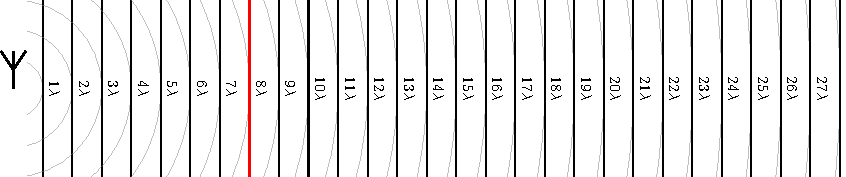
\includegraphics{../pictures/plana_0.pdf}
    \caption*{Fonte: Autor.}
    \label{fig:plana_0}
\end{figure}

% {Trigonometria}

Tomando agora um par de antenas separadas por uma distância fixa \ac{d}, torna-se viável fazer a análise trigonométrica entre as antenas e a frente de onda incidente, onde essa distância \ac{d} será a hipotenusa do triângulo retângulo formado.
Para realizar esta análise, ainda é necessário conhecer uma segunda dimensão do triângulo retângulo envolvido, esta é obtida da defasagem \ac{DeltaPhi} dos sinais incidentes nas antenas, conforme apresentado na \autoref{eq:defasagem}.
A \autoref{fig:AoA} apresenta quatro casos de chegada do sinal de \ac{RF} em um par de antenas.


% Relacao trigonometrica de defasagem e angulo do sinal
\begin{equation} \label{eq:defasagem}
    \ac{d} \cdot
    \cos\left(\textcolor{Purple}{\ac{betak}}\right) =
    \ac{lambda} \cdot
    \frac{\ac{DeltaPhi}}{2 \pi}
\end{equation}


É importante ressaltar que um sistema com um único par de antenas não é suficiente para determinar completamente o \ac{thetaAoA}, já que o valor calculado de \textcolor{Purple}{\ac{betak}} é igual para casos simétricos em relação ao par de antenas, criando um caso de ambiguidade.
As Figuras \ref{fig:AoA:1} e \ref{fig:AoA:2} apresentam exemplos de diferentes valores de \ac{thetaAoA} para o mesmo valor de \textcolor{Purple}{\ac{betak}}.
Existem ainda dois casos notáveis, onde o sinal chega alinhado ao par de antenas ou perpendicular a elas, apresentados respectivamente nas Figuras \ref{fig:AoA:3} e \ref{fig:AoA:4}.

\begin{figure}
    \caption{Diferentes valores de \ac{thetaAoA} para sinal incidente em par de antenas, sistema com ângulo $\textcolor{cmyk_M}{\ac{alphak}}=\SI{20}{\degree}$ em relação à referência.}
    \label{fig:AoA}

    \hfill
    \begin{subfigure}[b]{0.45\textwidth}
        \centering
        \caption{$ \ac{thetaAoA} = \SI{60}{\degree} $, $ \textcolor{Purple}{\ac{betak}} = \SI{40}{\degree} $}
        % \resizebox{!}{0.7\textheight}{%
\begin{circuitikz}[american, voltage shift=0.5, line width=0.5, every node/.style={font = {\footnotesize\bfseries}}]

    \def\wavelength{3.5}
    \pgfmathsetmacro\d{0.5*\wavelength}

    \def\antennaAngle{20}
    \pgfmathsetmacro\signalAngle{\antennaAngle+40}

    \def\closeRange{9}
    \def\farRange{\closeRange+13}

	\def\NAntennas{3}
	\pgfmathsetmacro\AngleAntennas{360/\NAntennas}
	\def\ShiftAngleAntennas{-90}

	\pgfmathsetmacro\RhoAntennas{\d/(2*sin(180/\NAntennas))}

    \def\centerarc(#1)(#2:#3:#4)% Syntax: [draw options] (center) (initial angle:final angle:radius)
    { ($(#1)+({#4*cos(#2)},{#4*sin(#2)})$) arc (#2:#3:#4) }

    \def\coordref[#1](#2){%

        \coordinate(sysref) at (#2);

        \draw[#1, -latex] (sysref) ++(-0.4,-0.3) -- ++(0.9,0) node[midway, below]{$x$};
        \draw[#1, -latex] (sysref) ++(-0.3,-0.4) -- ++(0,0.9) node[midway, left]{$y$};
        \draw[#1, -latex] \centerarc(sysref)(-90:180:0.25);
        \draw[#1] (sysref) node{$+$}
    }

    \coordinate (bottomleft) at (-3.5,-1);
    \coordinate (topright) at (3.5,5);


    % \draw[Red,dashed] (bottomleft) rectangle (topright);
    \clip (bottomleft) rectangle (topright);

    \coordinate (O) at (0,0);
    \coordinate (sourceAntenna) at (\signalAngle:\closeRange*\wavelength);
    % \draw [help lines, dashed] (bottomleft) grid (topright); % desenha grid
    % \draw [red] (O) node[draw,cross out] {}; % marca pont(0,0)

    % Circulo de antenas
	% \draw[densely dotted, opacity=0.25] (O) ++(90:\RhoAntennas) circle (\RhoAntennas);

    % Linhas do sinal de fundo
    \foreach \x [evaluate={\y=int((\x+\closeRange));\z=int((\x+\closeRange));}] in {-3,...,3} {
        \draw [black!75, very thin]
        (sourceAntenna) ++ (\signalAngle:-\z*\wavelength)
            % node[anchor=west, font = {\footnotesize\bfseries}]{$\y\lambda$}
        ($(sourceAntenna) + (\signalAngle:-\z*\wavelength) + ({10*cos(\signalAngle+90)},{10*sin(\signalAngle+90)})$)
            --
        ($(sourceAntenna) + (\signalAngle:-\z*\wavelength) - ({10*cos(\signalAngle+90)},{10*sin(\signalAngle+90)})$)
        % \draw [gray, thin] (sourceAntenna) circle (\z)
        ;
    }

    % Antenas
    \draw[thick, cmyk_R] (O) node[dinantenna] (A00) {} ;
    % \draw[thick, cmyk_G, opacity=0.75] (O) ++(60:\d) node[dinantenna] (A0d) {} node [below] {$A_{k+2}$};
    \draw[thick, cmyk_B] (O) ++(\antennaAngle:\d) node[dinantenna] (Ad0) {} ;

    \draw[very thin, Black!50, -latex] % Desenha eixo X
        (-3,0) -- (3,0) node[below left] {$x$}
    ;

    % Ângulo alpha entre antenas
    \draw[thin, cmyk_M]
        \centerarc(O)(0:\antennaAngle:0.3)
        node [above, inner sep=3pt] {$\alpha$}
    ;


    % Desenha senoide de fundo
    \draw[Goldenrod, domain=-8:8, samples=100]
        (A00) ++(\signalAngle+90:0.5*\wavelength) coordinate(signalAux)
        plot[shift={(signalAux)}, rotate=\signalAngle]({\x},{cos(\x * pi * 2 / \wavelength r)})
    ;

    % Direção do sinal
    \draw[very thick, dashed, -latex, Goldenrod]
        % (A00) ++(1.5*\d,0) ++ (\signalAngle:-0.5*\d) -- coordinate(angleArrow) ++(\signalAngle:\d)
        (A00) ++(-2,0) ++ (\signalAngle:-0.25*\d) -- coordinate(angleArrow) ++ (\signalAngle:0.5*\d) --++(\signalAngle:0.25*\d)
    ;
    % Angulo Theta do sinal
    \draw[thin]
        (angleArrow) ++ (0.4, 0) node [below,inner sep=2pt] {$\theta_\text{\ac{AoA}}$}
        \centerarc(angleArrow)(0:\signalAngle:0.4)
    ;

    % Triangulo retângulo + quadradinho
    \draw[Black]

        (A00) --++($({\signalAngle-90}:{\d*sin(\signalAngle-\antennaAngle)})$) coordinate (pontoTriangulo) -- (Ad0) -- (A00)

        (pontoTriangulo)
          ++(\signalAngle:0.125)
        --++(\signalAngle+90:0.125)
        --++(\signalAngle+180:0.125)
    ;

    % Arco do angulo beta
    \draw[thin, Purple]
        (Ad0) ++ (180+\antennaAngle:0.4) node[above, inner sep=3pt] {$\beta$}
        \centerarc(Ad0)(180+\antennaAngle:180+\signalAngle:0.4)
    ;

    % Distânci d entre antenas
    \draw[latex-latex]
        ($(A00)+(0,1)$) -- ($(Ad0)+(0,1)$) node [midway, fill=white, circle, inner sep=1pt] {$d$}
    ;

    \newcommand\CircleRadius{3cm}
    %   \draw (0,0) circle (\CircleRadius);
    % special method of noting the position of a point
    \coordinate (P) at (50:\CircleRadius);

\end{circuitikz}
% }


        % 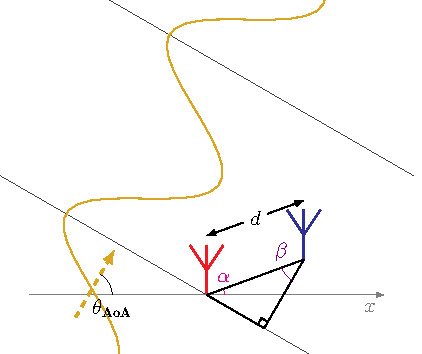
\includegraphics{../pictures/AoA_1.pdf}
        \label{fig:AoA:1}
    \end{subfigure}
    \hfill
    \begin{subfigure}[b]{0.45\textwidth}
        \centering
        \caption{$ \ac{thetaAoA} = \SI{-20}{\degree} $, $ \textcolor{Purple}{\ac{betak}} = \SI{40}{\degree} $}
            % \resizebox{!}{0.7\textheight}{%
    \begin{circuitikz}[american, voltage shift=0.5, line width=0.5,every node/.style={font = {\footnotesize\bfseries}}]

        \def\wavelength{3.5}
        \def\d{0.5*\wavelength}

        \def\antennaAngle{210}

        \def\closeRange{9}
        \def\farRange{\closeRange+13}

        \def\centerarc[#1](#2)(#3:#4:#5)% Syntax: [draw options] (center) (initial angle:final angle:radius)
        { \draw[#1] ($(#2)+({#5*cos(#3)},{#5*sin(#3)})$) arc (#3:#4:#5) node[midway,anchor=west] {$\beta$}; }


        \coordinate (O) at (0,0);
        \coordinate (antenna) at (\antennaAngle:\closeRange*\wavelength);
        % \draw [help lines, dashed] (-5,-3) grid (5,3); % desenha grid
        % \draw [red] (O) node[draw,cross out] {}; % marca pont(0,0) 
        
        % \draw (-6.8,-4) rectangle (6.8,4);
        \clip (-3.5,-3.5) rectangle (3.5,3.5);

        % \draw[thick]
        %     (antenna) node[dinantenna]{}
        % ;
        
        \foreach \x [evaluate={\y=int((\x+\closeRange));\z=int((\x+\closeRange));}] in {-3,...,3} {
            \draw [black, thin] 
            (antenna) ++ (\antennaAngle:-\z*\wavelength)
                % node[anchor=west, font = {\footnotesize\bfseries}]{$\y\lambda$}
            ($(antenna) + (\antennaAngle:-\z*\wavelength) + ({10*cos(\antennaAngle+90)},{10*sin(\antennaAngle+90)})$)
                -- 
            ($(antenna) + (\antennaAngle:-\z*\wavelength) - ({10*cos(\antennaAngle+90)},{10*sin(\antennaAngle+90)})$);
            % \draw [gray, thin] (antenna) circle (\z);
        }
        
        \draw[thick]
            (0,0)  node[Green, dinantenna] (A00) {}
            % (0,\d) node[Blue,  dinantenna] (A0d) {}
            (\d,0) node[Red,   dinantenna] (Ad0) {}
        ;

        \draw[very thick, dashed, -latex]
            (A00) ++(-\d,0) coordinate(aux) ++(\antennaAngle:0.5*\d) -- ++(\antennaAngle:-\d)
        ;

        
        \draw[Goldenrod, domain=-8:8, samples=100] plot[shift={(aux)}, rotate=\antennaAngle]({\x},{sin(\x * pi * 2 / \wavelength r)});
        
        \draw[thin, opacity=0.5]
            (A00) ++ ($({\antennaAngle-90}:{\d*sin(\antennaAngle)})$) -- (Ad0) -- (A00)

            ($({\antennaAngle-90}:{\d*sin(\antennaAngle)})$) 
              ++(\antennaAngle+180:0.125)
            --++(\antennaAngle-90:0.125)
            --++(\antennaAngle:0.125)

            
        ;

        \centerarc[thin, opacity=0.5](A00)(\antennaAngle+90:360:0.4)

        \draw[latex-latex]
            ($(A00)+(0,1)$) -- ($(Ad0)+(0,1)$) node [midway, fill=white] {$d$}
        ;
        


        % \foreach \x in {0,60,...,300} {
        %     \draw[thick] (\x:1 cm) -- (\x + 60:1 cm);
            
        %     \draw (\x + 30:1.732 cm) node[Gray, circ]{};
        %     \draw[Gray, dashed] (\x:1 cm) -- ++(\x: 0.9cm);
        %     \draw[Gray, dotted]
        %     %     % (\x:1 cm) arc (\x+240:\x+180:1cm)
        %         (\x:1 cm) arc [start angle=\x+120, delta angle=110, radius=1cm]
        %         (\x:1 cm) arc [start angle=\x+120, delta angle=-50, radius=1cm]
        %     ;
        % }
    
        % \draw (0,0) node [circ] {} node [below left,font={\scriptsize\bfseries}] {BS};
        % \draw[thick, densely dotted] (0,0) circle (1cm);
        
        % \draw[-latex] (0,0) -- (0:1cm) node[midway, below] {$R_c$};
        % \draw[-latex] (0,0) -- (90:0.866cm) node[midway, left] {$R$};
            
    \end{circuitikz}
  % }


        % 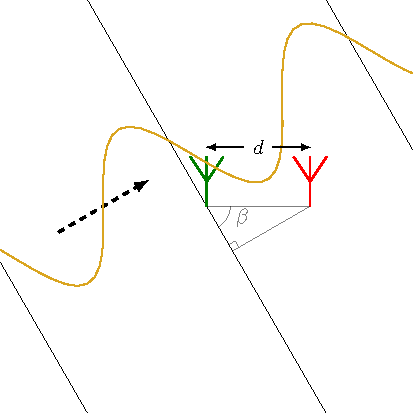
\includegraphics{../pictures/AoA_2.pdf}
        \label{fig:AoA:2}
    \end{subfigure}
    \hfill

    \vspace{\floatsep}

    \hfill
    \begin{subfigure}[b]{0.45\textwidth}
        \centering
        \caption{$ \ac{thetaAoA}=\SI{110}{\degree} $, $ \textcolor{Purple}{\ac{betak}} = \SI{90}{\degree} $}
            % \resizebox{!}{0.7\textheight}{%
    \begin{circuitikz}[american, voltage shift=0.5, line width=0.5,every node/.style={font = {\footnotesize\bfseries}}]

        \def\wavelength{3.5}
        \def\d{0.5*\wavelength}


        \def\antennaAngle{180}
        \def\closeRange{9}
        \def\farRange{\closeRange+13}

        \def\centerarc[#1](#2)(#3:#4:#5)% Syntax: [draw options] (center) (initial angle:final angle:radius)
        { \draw[#1] ($(#2)+({#5*cos(#3)},{#5*sin(#3)})$) arc (#3:#4:#5) node[midway,anchor=west] {$\beta$}; }


        \coordinate (O) at (0,0);
        \coordinate (antenna) at (\antennaAngle:\closeRange*\wavelength);
        % \draw [help lines, dashed] (-5,-3) grid (5,3); % desenha grid
        % \draw [red] (O) node[draw,cross out] {}; % marca pont(0,0) 
        
        % \draw (-6.8,-4) rectangle (6.8,4);
        \clip (-3.5,-3.5) rectangle (3.5,3.5);

        % \draw[thick]
        %     (antenna) node[dinantenna]{}
        % ;
        
        \foreach \x [evaluate={\y=int((\x+\closeRange));\z=int((\x+\closeRange));}] in {-3,...,3} {
            \draw [black, thin] 
            (antenna) ++ (\antennaAngle:-\z*\wavelength)
                % node[anchor=west, font = {\footnotesize\bfseries}]{$\y\lambda$}
            ($(antenna) + (\antennaAngle:-\z*\wavelength) + ({10*cos(\antennaAngle+90)},{10*sin(\antennaAngle+90)})$)
                -- 
            ($(antenna) + (\antennaAngle:-\z*\wavelength) - ({10*cos(\antennaAngle+90)},{10*sin(\antennaAngle+90)})$);
            % \draw [gray, thin] (antenna) circle (\z);
        }
        
        \draw[thick]
            (0,0)  node[Green, dinantenna] (A00) {}
            % (0,\d) node[Blue,  dinantenna] (A0d) {}
            (\d,0) node[Red,   dinantenna] (Ad0) {}
        ;

        \draw[very thick, dashed, -latex]
            (A00) ++(-\d,0) coordinate(aux) ++(\antennaAngle:0.5*\d) -- ++(\antennaAngle:-\d)
        ;

        
        \draw[Goldenrod, domain=-8:8, samples=100] plot[shift={(aux)}, rotate=\antennaAngle]({\x},{cos(\x * pi * 2 / \wavelength r)});
        % \draw[thin, densely dotted]
        %     (A00) ++ ($({\antennaAngle-90}:{\d*sin(\antennaAngle)})$) -- (Ad0) -- (A00)

        %     ($({\antennaAngle-90}:{\d*sin(\antennaAngle)})$) 
        %       ++(\antennaAngle+180:0.25)
        %     --++(\antennaAngle-90:0.25)
        %     --++(\antennaAngle:0.25)

            
        % ;

        % \centerarc[thin, densely dotted](A00)(\antennaAngle+90:360:0.4)

        \draw[latex-latex]
            ($(A00)+(0,1)$) -- ($(Ad0)+(0,1)$) node [midway, fill=white] {$d$}
        ;

        % \draw[color=Blue, samples=100, domain=-4:4, smooth]
        %     (A00)++(-\d,0)
        %     % plot[rotate=\antennaAngle] ({\x},{sin((\x r)*0.31830)})
        % ;


        % \foreach \x in {0,60,...,300} {
        %     \draw[thick] (\x:1 cm) -- (\x + 60:1 cm);
            
        %     \draw (\x + 30:1.732 cm) node[Gray, circ]{};
        %     \draw[Gray, dashed] (\x:1 cm) -- ++(\x: 0.9cm);
        %     \draw[Gray, dotted]
        %     %     % (\x:1 cm) arc (\x+240:\x+180:1cm)
        %         (\x:1 cm) arc [start angle=\x+120, delta angle=110, radius=1cm]
        %         (\x:1 cm) arc [start angle=\x+120, delta angle=-50, radius=1cm]
        %     ;
        % }
    
        % \draw (0,0) node [circ] {} node [below left,font={\scriptsize\bfseries}] {BS};
        % \draw[thick, densely dotted] (0,0) circle (1cm);
        
        % \draw[-latex] (0,0) -- (0:1cm) node[midway, below] {$R_c$};
        % \draw[-latex] (0,0) -- (90:0.866cm) node[midway, left] {$R$};
            
    \end{circuitikz}
  % }


        % 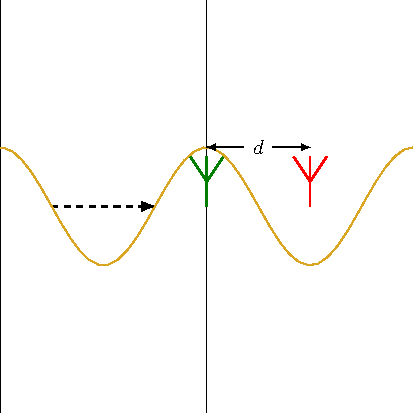
\includegraphics{../pictures/AoA_3.pdf}
        \label{fig:AoA:3}
    \end{subfigure}
    \hfill
    \begin{subfigure}[b]{0.45\textwidth}
        \centering
        \caption{$ \ac{thetaAoA}=\SI{20}{\degree} $, $ \textcolor{Purple}{\ac{betak}} = \SI{0}{\degree} $}
        % \resizebox{!}{0.7\textheight}{%
\begin{circuitikz}[american, voltage shift=0.5, line width=0.5, every node/.style={font = {\footnotesize\bfseries}}]

    \def\wavelength{3.5}
    \pgfmathsetmacro\d{0.5*\wavelength}

    \def\antennaAngle{20}
    \def\signalAngle{\antennaAngle}

    \def\closeRange{9}
    \def\farRange{\closeRange+13}

	\def\NAntennas{3}
	\pgfmathsetmacro\AngleAntennas{360/\NAntennas}
	\def\ShiftAngleAntennas{-90}

	\pgfmathsetmacro\RhoAntennas{\d/(2*sin(180/\NAntennas))}

    \def\centerarc(#1)(#2:#3:#4)% Syntax: [draw options] (center) (initial angle:final angle:radius)
    { ($(#1)+({#4*cos(#2)},{#4*sin(#2)})$) arc (#2:#3:#4) }

    \def\coordref[#1](#2){%

        \coordinate(sysref) at (#2);

        \draw[#1, -latex] (sysref) ++(-0.4,-0.3) -- ++(0.9,0) node[midway, below]{$x$};
        \draw[#1, -latex] (sysref) ++(-0.3,-0.4) -- ++(0,0.9) node[midway, left]{$y$};
        \draw[#1, -latex] \centerarc(sysref)(-90:180:0.25);
        \draw[#1] (sysref) node{$+$}
    }

    \coordinate (bottomleft) at (-3.5,-1);
    \coordinate (topright) at (3.5,5);


    % \draw[Red,dashed] (bottomleft) rectangle (topright);
    \clip (bottomleft) rectangle (topright);

    \coordinate (O) at (0,0);
    \coordinate (sourceAntenna) at (\signalAngle:\closeRange*\wavelength);
    % \draw [help lines, dashed] (bottomleft) grid (topright); % desenha grid
    % \draw [red] (O) node[draw,cross out] {}; % marca pont(0,0)

    % Circulo de antenas
	% \draw[densely dotted, opacity=0.25] (O) ++(90:\RhoAntennas) circle (\RhoAntennas);

    % Linhas do sinal de fundo
    \foreach \x [evaluate={\y=int((\x+\closeRange));\z=int((\x+\closeRange));}] in {-3,...,3} {
        \draw [black!75, very thin]
        (sourceAntenna) ++ (\signalAngle:-\z*\wavelength)
            % node[anchor=west, font = {\footnotesize\bfseries}]{$\y\lambda$}
        ($(sourceAntenna) + (\signalAngle:-\z*\wavelength) + ({10*cos(\signalAngle+90)},{10*sin(\signalAngle+90)})$)
            --
        ($(sourceAntenna) + (\signalAngle:-\z*\wavelength) - ({10*cos(\signalAngle+90)},{10*sin(\signalAngle+90)})$)
        % \draw [gray, thin] (sourceAntenna) circle (\z)
        ;
    }

    % Antenas
    \draw[thick, cmyk_R] (O) node[dinantenna] (A00) {} ;
    % \draw[thick, cmyk_G, opacity=0.75] (O) ++(60:\d) node[dinantenna] (A0d) {} node [below] {$A_{k+2}$};
    \draw[thick, cmyk_B] (O) ++(\antennaAngle:\d) node[dinantenna] (Ad0) {} ;

    \draw[very thin, Black!50, -latex] % Desenha eixo X
        (-3,0) -- (3,0) node[below left] {$x$}
    ;

    % Ângulo alpha entre antenas
    \draw[thin, cmyk_M]
		(0.3,0) node [below, inner sep=3pt] {$\alpha$}
		\centerarc(O)(0:\antennaAngle:0.3)
    ;


    % Desenha senoide de fundo
    \draw[Goldenrod, domain=-8:8, samples=100]
        (A00) ++(\signalAngle+90:0.75*\wavelength) coordinate(signalAux)
        plot[shift={(signalAux)}, rotate=\signalAngle]({\x},{cos(\x * pi * 2 / \wavelength r)})
    ;

    % Direção do sinal
    \draw[very thick, dashed, -latex, Goldenrod]
        % (A00) ++(1.5*\d,0) ++ (\signalAngle:-0.25*\d) -- coordinate(angleArrow) ++(\signalAngle:0.85*\d)
        (A00) ++(-2,0) ++ (\signalAngle:-0.25*\d) -- coordinate(angleArrow) ++ (\signalAngle:0.5*\d) --++(\signalAngle:0.25*\d)
    ;
    % Angulo Theta do sinal
    \draw[thin]
        (angleArrow) ++ (0.4, 0) node [below,inner sep=2pt] {$\theta_\text{\ac{AoA}}$}
        \centerarc(angleArrow)(0:\signalAngle:0.4)
    ;

    % Triangulo retângulo + quadradinho
    \draw[Black]

    %     % (A00) --++($({\signalAngle-90}:{\d*sin(\signalAngle-\antennaAngle)})$) coordinate (pontoTriangulo) --
		(Ad0) -- (A00)

    %     % (pontoTriangulo)
    %     %   ++(\signalAngle:0.125)
    %     % --++(\signalAngle+90:0.125)
    %     % --++(\signalAngle+180:0.125)
    ;

    % % Arco do angulo beta
    % \draw[thin]
    %     \centerarc(Ad0)(180+\antennaAngle:180+\signalAngle:0.4) node[below, inner sep=3pt] {$\beta$}
    % ;

    % Distânci d entre antenas
    \draw[latex-latex]
        ($(A00)+(0,1)$) -- ($(Ad0)+(0,1)$) node [midway, fill=white, circle, inner sep=1pt] {$d$}
    ;

    \newcommand\CircleRadius{3cm}
    %   \draw (0,0) circle (\CircleRadius);
    % special method of noting the position of a point
    \coordinate (P) at (50:\CircleRadius);

\end{circuitikz}
% }


        % 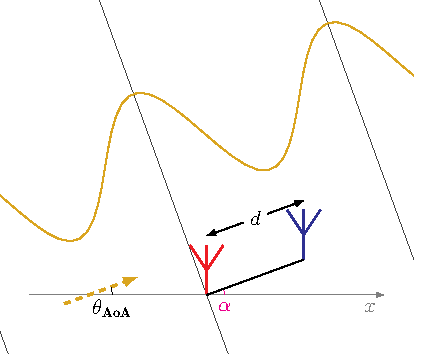
\includegraphics{../pictures/AoA_4.pdf}
        \label{fig:AoA:4}
    \end{subfigure}
    \hfill

    \caption*{Fonte: Autor.}
\end{figure}

% {Distância entre antenas}

A escolha da distância \ac{d} entre as antenas deve ser feita de forma a otimizar a resolução da medida de defasagem, com a maior distância possível. Porém é necessário evitar ambiguidades na análise, por se tratar de um sinal periódico, o valor se repetirá a cada \ac{lambda}, e terá valores simétricos quando $\ac{d} > \sfrac{\ac{lambda}}{2}$, ilustrado na \autoref{fig:AoA_d:fail}.
Adota-se então $\ac{d}=\sfrac{\ac{lambda}}{2}$, conforme apresentado na \autoref{fig:AoA_d:ok} e \autoref{eq:distancia} \cite{bensky2016wireless, horst2021localization, Schssel2016AngleOA}.

\begin{figure}[htbp]
    \caption{Diferentes valores para \ac{d}.}
    \label{fig:AoA_d}

    \hfill
    \begin{subfigure}[b]{0.45\textwidth}
        \centering
        \caption{$\ac{d} > \sfrac{\ac{lambda}}{2}$}
            % \resizebox{!}{0.7\textheight}{%
    \begin{circuitikz}[american, voltage shift=0.5, line width=0.5,every node/.style={font = {\footnotesize\bfseries}}]

        \def\wavelength{4}
        \def\d{0.5*\wavelength}


        \def\antennaAngle{120}
        \def\closeRange{9}
        \def\farRange{\closeRange+13}

        \def\centerarc[#1](#2)(#3:#4:#5)% Syntax: [draw options] (center) (initial angle:final angle:radius)
        { \draw[#1] ($(#2)+({#5*cos(#3)},{#5*sin(#3)})$) arc (#3:#4:#5) node[midway,anchor=west] {$\beta$}; }


        \coordinate (O) at (0,0);
        \coordinate (antenna) at (\antennaAngle:\closeRange*\wavelength);
        % \draw [help lines, dashed] (-3,-3) grid (3,3); % desenha grid
        % \draw [red] (O) node[draw,cross out] {}; % marca pont(0,0)

        % \draw (-6.8,-4) rectangle (6.8,4);
        \clip (-1,-1.1) rectangle (5,1.1);


        \draw[thick]
            (0,0)  node[cmyk_B, dinantenna] (A00) {}
            % (0,\d) node[Blue,  dinantenna] (A0d) {}
            (1.2*\d,0) node[cmyk_R,   dinantenna] (Ad0) {}
            (0.8*\d,0) node[cmyk_R,   dinantenna, opacity=0.2] (Ad0_phantom) {}
        ;

        % \draw[Goldenrod, domain=-3:3, samples=100] plot[shift={(-1,-1)}, rotate=30]({\x},{sin(\x * pi * 2 / \wavelength r)});
        \draw[Goldenrod, domain=-3:6, samples=50]
            plot ({\x},{cos(\x * pi * 2 / \wavelength r)})
        ;

        \draw[Black, dashed, domain=-3:6, samples=2]
            plot[Black, thin, dashed, samples=2] (\x,0)
        ;

        \draw [densely dotted, cmyk_R]
            (Ad0_phantom) --
            ++(0,{cos(1.2*\d * pi * 2 / \wavelength r)}) --
            ++({0.4*\d},0) --
            (Ad0)
        ;

    \end{circuitikz}
  % }
        % 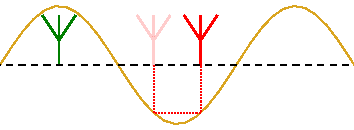
\includegraphics{../pictures/AoA_0_fail.pdf}
        \label{fig:AoA_d:fail}
    \end{subfigure}
    \hfill
    \begin{subfigure}[b]{0.45\textwidth}
        \centering
        \caption{$\ac{d} = \sfrac{\ac{lambda}}{2}$}
            % \resizebox{!}{0.7\textheight}{%
    \begin{circuitikz}[american, voltage shift=0.5, line width=0.5,every node/.style={font = {\footnotesize\bfseries}}]

        \def\wavelength{4}
        \def\d{0.5*\wavelength}


        \def\antennaAngle{120}
        \def\closeRange{9}
        \def\farRange{\closeRange+13}

        \def\centerarc[#1](#2)(#3:#4:#5)% Syntax: [draw options] (center) (initial angle:final angle:radius)
        { \draw[#1] ($(#2)+({#5*cos(#3)},{#5*sin(#3)})$) arc (#3:#4:#5) node[midway,anchor=west] {$\beta$}; }


        \coordinate (O) at (0,0);
        \coordinate (antenna) at (\antennaAngle:\closeRange*\wavelength);
        % \draw [help lines, dashed] (-3,-3) grid (3,3); % desenha grid
        % \draw [red] (O) node[draw,cross out] {}; % marca pont(0,0) 
        
        % \draw (5,1.25) rectangle (-1,-1.1);
        \clip (5,1.25) rectangle (-1,-1.1);

        
        % \draw[Goldenrod, domain=-3:3, samples=100] plot[shift={(-1,-1)}, rotate=30]({\x},{sin(\x * pi * 2 / \wavelength r)});
        \draw[Goldenrod, domain=-3:6, samples=50] 
            plot ({\x},{cos(\x * pi * 2 / \wavelength r)})
        ;
        
        \draw[Black, dashed, domain=-3:6, samples=2] 
            plot[Black, thin, dashed, samples=2] (\x,0)
        ;
        
        
        % \pause
        \draw[thick]
            (0,0)  node[Green, dinantenna] (A00) {}
            % (0,\d) node[Blue,  dinantenna] (A0d) {}
            % (\d,0) node[Red,   dinantenna] (Ad0) {}
        ;
        
        % \pause
        \draw[thick]
            % (0,0)  node[Green, dinantenna] (A00) {}
            % (0,\d) node[Blue,  dinantenna] (A0d) {}
            (\d,0) node[Red,   dinantenna] (Ad0) {}
        ;

        \draw[latex-latex]
            ($(A00)+(0,1.1)$) -- ++(\wavelength,0) node [midway, fill=white] {$\lambda$}
        ;
    % \visible<7->{
        \draw[latex-latex]
            ($(A00)+(0,-0.1)$) -- ++(0.5*\wavelength,0) node [midway, fill=white, fill opacity=0.75, anchor=north] {$d = \sfrac{\lambda}{2}$}
        ;
    % }
            
    \end{circuitikz}
  % }
        % 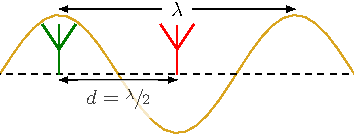
\includegraphics{../pictures/AoA_0.pdf}
        \label{fig:AoA_d:ok}
    \end{subfigure}
    \hfill

    \caption*{Fonte: Autor.}
\end{figure}

\begin{equation} \label{eq:distancia} % Distancia entre par de antenas
    \ac{d} = \frac{\ac{lambda}}{2}
\end{equation}

% % {Ambiguidade simétrica}

Para contornar a ambiguidade de simetria, é possível adicionar mais antenas à malha.
O conjunto de \ac{Nant} antenas deve respeitar a distância \ac{d} entre as antenas de um par, e pode ser disposto como um polígono regular com \ac{Nant} lados de tamanho \ac{d}, onde cada antena está em um vértice.
A \autoref{fig:antennas} apresenta exemplos dessa disposição de antenas, note que valores pares de \ac{Nant} implicam que existirão pares de antenas paralelos, que resultam em leituras redundantes.

\begin{figure}[htbp]
    \centering
    \caption{Diferentes distribuições de antenas.}
    \label{fig:antennas}

    \hfill
    \begin{subfigure}[c]{0.4\textwidth}
        \centering
        \caption{$ \ac{Nant} = 3 $.}
        % % \resizebox{!}{0.7\textheight}{%
\begin{circuitikz}[american, voltage shift=0.5, line width=0.5,every node/.style={font = {\footnotesize\bfseries}}]

    \def\wavelength{8}
    \pgfmathsetmacro\d{0.5*\wavelength}

    \def\signalAngle{75}
    \def\antennaAngle{120}

    \def\closeRange{9}
    \def\farRange{\closeRange+13}

	\def\NAntennas{3}
	\pgfmathsetmacro\AngleAntennas{360/\NAntennas}
	\def\ShiftAngleAntennas{-90}

	\pgfmathsetmacro\RhoAntennas{\d/(2*sin(180/\NAntennas))}

    \def\centerarc(#1)(#2:#3:#4)% Syntax: [draw options] (center) (initial angle:final angle:radius)
    { ($(#1)+({#4*cos(#2)},{#4*sin(#2)})$) arc (#2:#3:#4) }

    \def\coordref[#1](#2){%

        \coordinate(sysref) at (#2);

        \draw[#1, -latex] (sysref) ++(-0.4,-0.3) -- ++(0.9,0) node[midway, below]{$x$};
        \draw[#1, -latex] (sysref) ++(-0.3,-0.4) -- ++(0,0.9) node[midway, left]{$y$};
        \draw[#1, -latex] \centerarc(sysref)(-90:180:0.25);
        \draw[#1] (sysref) node{$+$}
    }

    \coordinate (bottomleft) at (-3,-3);
    \coordinate (topright) at (3,3);


    % \draw[Red,dashed] (bottomleft) rectangle (topright);
    \clip (bottomleft) rectangle (topright);

    \coordinate (O) at (0,0);
    \coordinate (sourceAntenna) at (\signalAngle:\closeRange*\wavelength);
    % \draw [help lines, dashed] (bottomleft) grid (topright); % desenha grid
    % \draw [red] (O) node[draw,cross out] {}; % marca pont(0,0)

	\draw[densely dotted] (O) circle (\RhoAntennas);

    \draw[thick, cmyk_G] (O) ++(1*\AngleAntennas+\ShiftAngleAntennas:\RhoAntennas) node[dinantenna] (A1) {} node [above right] {$A_{1}$};
    \draw[thick, cmyk_B] (O) ++(2*\AngleAntennas+\ShiftAngleAntennas:\RhoAntennas) node[dinantenna] (A2) {} node [above left] {$A_{2}$};
    \draw[thick, cmyk_R] (O) ++(3*\AngleAntennas+\ShiftAngleAntennas:\RhoAntennas) node[dinantenna] (A3) {};

	\coordinate (A1_2) at ($(A1)!0.5!(A2)$);

	\draw[Black!25, dotted]
		(A1) --
		(A3) --
		(A2)
	;

	\draw[Black!50, densely dotted]
		(O) --
		(A2) --
		(A1_2)
	;

	\draw
		(A1) --
		(O) --
		(A1_2) --
		(A1)
	;

	\draw
         (A1_2)
           ++(0:0.125)
         --++(-90:0.125)
         --++(+180:0.125)
	;

	\node at (O) {\tiny\textbullet};

	\draw
		(O) ++(90:0.3) node[left, inner sep=1.5pt] {$\textstyle \frac{\pi}{N_\text{ant}}$}
		\centerarc(O)(1*\AngleAntennas+\ShiftAngleAntennas:90:0.3)
	;


    % Distânci d entre antenas
    \draw[latex-latex]
        ($(A1)+(0,1)$) -- ($(A2)+(0,1)$) node [midway, fill=white, circle, inner sep=1pt] {$d$}
    ;

    \draw[decorate, decoration={brace, amplitude=5pt}, thin]
    ($(A1)+({1*\AngleAntennas+\ShiftAngleAntennas-90}:0.1)$)
    -- coordinate (brace)
    ($(O)+({1*\AngleAntennas+\ShiftAngleAntennas-90}:0.1)$)
    ;

    \draw (brace) ++({1*\AngleAntennas+\ShiftAngleAntennas-90}:5pt)
        node[anchor=north west, circle, fill=white, inner sep=1pt] {$\rho$}
    ;

	\draw[decorate, decoration={brace, amplitude=5pt}, thin]
    ($(A1_2)+({90}:0.1)$)
    -- coordinate (brace)
    ($(A1)+({90}:0.1)$)
    ;

    \draw (brace) ++({90}:5pt)
        node[anchor=south, circle, inner sep=1pt] {$\sfrac{d}{2}$}
    ;

    % \coordref[Black!25](3.5,0);

\end{circuitikz}
% }


        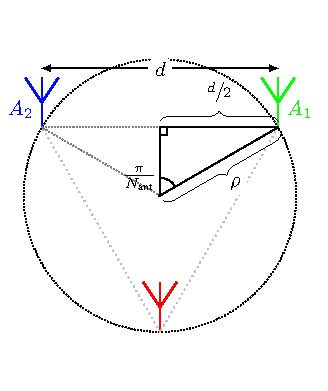
\includegraphics{../pictures/antennas_3.pdf}
        \label{fig:antennas:3}
    \end{subfigure}
    \hfill
    \begin{subfigure}[c]{0.575\textwidth}
        \centering
        \caption{$ \ac{Nant} = 6 $.}
        % % \resizebox{!}{0.7\textheight}{%
\begin{circuitikz}[american, voltage shift=0.5, line width=0.5,every node/.style={font = {\footnotesize\bfseries}}]

    \def\wavelength{8}
    \pgfmathsetmacro\d{0.5*\wavelength}

    \def\signalAngle{75}
    \def\antennaAngle{120}

    \def\closeRange{9}
    \def\farRange{\closeRange+13}

	\def\NAntennas{6}
	\pgfmathsetmacro\AngleAntennas{360/\NAntennas}
	\pgfmathsetmacro\ShiftAngleAntennas{-90+1.5*\AngleAntennas}

	\pgfmathsetmacro\RhoAntennas{\d/(2*sin(180/\NAntennas))}

    \def\centerarc(#1)(#2:#3:#4)% Syntax: [draw options] (center) (initial angle:final angle:radius)
    { ($(#1)+({#4*cos(#2)},{#4*sin(#2)})$) arc (#2:#3:#4) }

    \def\coordref[#1](#2){%

        \coordinate(sysref) at (#2);

        \draw[#1, -latex] (sysref) ++(-0.4,-0.3) -- ++(0.9,0) node[midway, below]{$x$};
        \draw[#1, -latex] (sysref) ++(-0.3,-0.4) -- ++(0,0.9) node[midway, left]{$y$};
        \draw[#1, -latex] \centerarc(sysref)(-90:180:0.25);
        \draw[#1] (sysref) node{$+$}
    }

    \coordinate (bottomleft) at (-4.5,-4.5);
    \coordinate (topright) at (4.5,4.5);


    % \draw[Red,dashed] (bottomleft) rectangle (topright);
    \clip (bottomleft) rectangle (topright);

    \coordinate (O) at (0,0);
    \coordinate (sourceAntenna) at (\signalAngle:\closeRange*\wavelength);
    % \draw [help lines, dashed] (bottomleft) grid (topright); % desenha grid
    % \draw [red] (O) node[draw,cross out] {}; % marca pont(0,0)

	\draw[densely dotted] (O) circle (\RhoAntennas);

    \draw[thick, cmyk_G] (O) ++(1*\AngleAntennas+\ShiftAngleAntennas:\RhoAntennas) node[dinantenna] (A1) {} node [above right] {$A_{1}$};
    \draw[thick, cmyk_B] (O) ++(2*\AngleAntennas+\ShiftAngleAntennas:\RhoAntennas) node[dinantenna] (A2) {} node [above left] {$A_{2}$};
    \draw[thick, cmyk_R] (O) ++(3*\AngleAntennas+\ShiftAngleAntennas:\RhoAntennas) node[dinantenna] (A3) {};
    \draw[thick, cmyk_C] (O) ++(4*\AngleAntennas+\ShiftAngleAntennas:\RhoAntennas) node[dinantenna] (A4) {};
    \draw[thick, cmyk_M] (O) ++(5*\AngleAntennas+\ShiftAngleAntennas:\RhoAntennas) node[dinantenna] (A5) {};
    \draw[thick, DarkGoldenrod] (O) ++(6*\AngleAntennas+\ShiftAngleAntennas:\RhoAntennas) node[dinantenna] (A6) {};

	\coordinate (A1_2) at ($(A1)!0.5!(A2)$);

	\draw[Black!25, dotted]
		(A1) --
		(A6) --
		(A5) --
		(A4) --
		(A3) --
		(A2)
	;

	\draw[Black!50, densely dotted]
		(O) --
		(A2) --
		(A1_2)
	;

	\draw
		(A1) --
		(O) --
		(A1_2) --
		(A1)
	;

	\draw
         (A1_2)
           ++(0:0.125)
         --++(-90:0.125)
         --++(+180:0.125)
	;

	\node at (O) {\tiny\textbullet};

	\draw
		(O) ++(90:0.3) node[left, inner sep=1.5pt] {$\textstyle \frac{\pi}{N_\text{ant}}$}
		\centerarc(O)(1*\AngleAntennas+\ShiftAngleAntennas:90:0.3)
	;


    % Distânci d entre antenas
    \draw[latex-latex]
        ($(A1)+(0,1)$) -- ($(A2)+(0,1)$) node [midway, fill=white, circle, inner sep=1pt] {$d$}
    ;

    \draw[decorate, decoration={brace, amplitude=5pt}, thin]
    ($(A1)+({1*\AngleAntennas+\ShiftAngleAntennas-90}:0.1)$)
    -- coordinate (brace)
    ($(O)+({1*\AngleAntennas+\ShiftAngleAntennas-90}:0.1)$)
    ;

    \draw (brace) ++({1*\AngleAntennas+\ShiftAngleAntennas-90}:5pt)
        node[anchor=north west, circle, fill=white, inner sep=1pt] {$\rho$}
    ;

	\draw[decorate, decoration={brace, amplitude=5pt}, thin]
    ($(A1_2)+({90}:0.1)$)
    -- coordinate (brace)
    ($(A1)+({90}:0.1)$)
    ;

    \draw (brace) ++({90}:5pt)
        node[anchor=south, circle, inner sep=1pt] {$\sfrac{d}{2}$}
    ;

    % \coordref[Black!25](3.5,0);

\end{circuitikz}
% }


        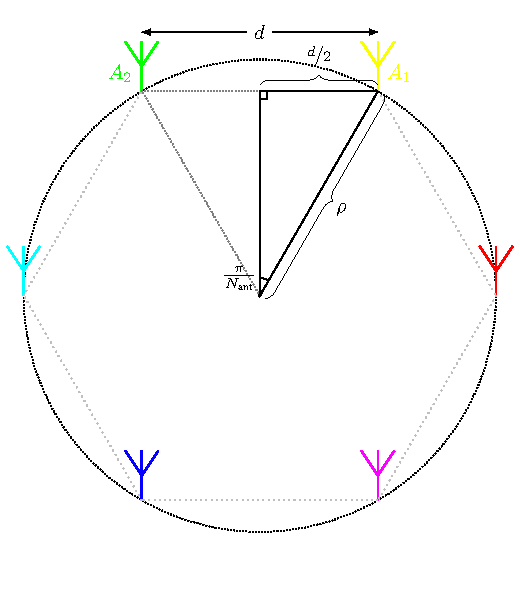
\includegraphics{../pictures/antennas_6.pdf}
        \label{fig:antennas:6}
    \end{subfigure}
    \hfill

    \vspace{\floatsep}

    \hfill
    \begin{subfigure}[c]{0.425\textwidth}
        \centering
        \caption{$ \ac{Nant} = 4 $.}
        % % \resizebox{!}{0.7\textheight}{%
\begin{circuitikz}[american, voltage shift=0.5, line width=0.5,every node/.style={font = {\footnotesize\bfseries}}]

    \def\wavelength{8}
    \pgfmathsetmacro\d{0.5*\wavelength}

    \def\signalAngle{75}
    \def\antennaAngle{120}

    \def\closeRange{9}
    \def\farRange{\closeRange+13}

	\def\NAntennas{4}
	\pgfmathsetmacro\AngleAntennas{360/\NAntennas}
	\pgfmathsetmacro\ShiftAngleAntennas{-90+0.5*\AngleAntennas}

	\pgfmathsetmacro\RhoAntennas{\d/(2*sin(180/\NAntennas))}

    \def\centerarc(#1)(#2:#3:#4)% Syntax: [draw options] (center) (initial angle:final angle:radius)
    { ($(#1)+({#4*cos(#2)},{#4*sin(#2)})$) arc (#2:#3:#4) }

    \def\coordref[#1](#2){%

        \coordinate(sysref) at (#2);

        \draw[#1, -latex] (sysref) ++(-0.4,-0.3) -- ++(0.9,0) node[midway, below]{$x$};
        \draw[#1, -latex] (sysref) ++(-0.3,-0.4) -- ++(0,0.9) node[midway, left]{$y$};
        \draw[#1, -latex] \centerarc(sysref)(-90:180:0.25);
        \draw[#1] (sysref) node{$+$}
    }

    \pgfmathsetmacro\vSize{\RhoAntennas + 1}
    \pgfmathsetmacro\hSize{\RhoAntennas + 0.4}

    \coordinate (bottomleft) at (-\hSize,-\vSize);
    \coordinate (topright) at (\hSize,\vSize);


    % \draw[Red,dashed] (bottomleft) rectangle (topright);
    \clip (bottomleft) rectangle (topright);

    \coordinate (O) at (0,0);
    \coordinate (sourceAntenna) at (\signalAngle:\closeRange*\wavelength);
    % \draw [help lines, dashed] (bottomleft) grid (topright); % desenha grid
    % \draw [red] (O) node[draw,cross out] {}; % marca pont(0,0)

	\draw[densely dotted] (O) circle (\RhoAntennas);

    \draw[thick, antena_4_1] (O) ++(1*\AngleAntennas+\ShiftAngleAntennas:\RhoAntennas) node[dinantenna] (A1) {} node [above right] {$A_{1}$};
    \draw[thick, antena_4_2] (O) ++(2*\AngleAntennas+\ShiftAngleAntennas:\RhoAntennas) node[dinantenna] (A2) {} node [above left] {$A_{2}$};
    \draw[thick, antena_4_3] (O) ++(3*\AngleAntennas+\ShiftAngleAntennas:\RhoAntennas) node[dinantenna] (A3) {};
    \draw[thick, antena_4_4] (O) ++(4*\AngleAntennas+\ShiftAngleAntennas:\RhoAntennas) node[dinantenna] (A4) {};
    % \draw[thick, cmyk_M] (O) ++(5*\AngleAntennas+\ShiftAngleAntennas:\RhoAntennas) node[dinantenna] (A5) {};

	\coordinate (A1_2) at ($(A1)!0.5!(A2)$);

	\draw[Black!25, dotted]
		(A1) --
		(A4) --
		(A3) --
		(A2)
	;

	\draw[Black!50, densely dotted]
		(O) --
		(A2) --
		(A1_2)
	;

	\draw
		(A1) --
		(O) --
		(A1_2) --
		(A1)
	;

	\draw
         (A1_2)
           ++(0:0.125)
         --++(-90:0.125)
         --++(+180:0.125)
	;

	\node at (O) {\tiny\textbullet};

	\draw
		(O) ++(90:0.3) node[left, inner sep=1.5pt] {$\textstyle \frac{\pi}{N_\text{ant}}$}
		\centerarc(O)(1*\AngleAntennas+\ShiftAngleAntennas:90:0.3)
	;


    % Distânci d entre antenas
    \draw[latex-latex]
        ($(A1)+(0,1)$) -- ($(A2)+(0,1)$) node [midway, fill=white, circle, inner sep=1pt] {$d$}
    ;

    \draw[decorate, decoration={brace, amplitude=5pt}, thin]
    ($(A1)+({1*\AngleAntennas+\ShiftAngleAntennas-90}:0.1)$)
    -- coordinate (brace)
    ($(O)+({1*\AngleAntennas+\ShiftAngleAntennas-90}:0.1)$)
    ;

    \draw (brace) ++({1*\AngleAntennas+\ShiftAngleAntennas-90}:5pt)
        node[anchor=north west, circle, fill=white, inner sep=1pt] {$\rho$}
    ;

	\draw[decorate, decoration={brace, amplitude=5pt}, thin]
    ($(A1_2)+({90}:0.1)$)
    -- coordinate (brace)
    ($(A1)+({90}:0.1)$)
    ;

    \draw (brace) ++({90}:5pt)
        node[anchor=south, circle, inner sep=1pt] {$\sfrac{d}{2}$}
    ;

    % \coordref[Black!25](3.5,0);

\end{circuitikz}
% }


        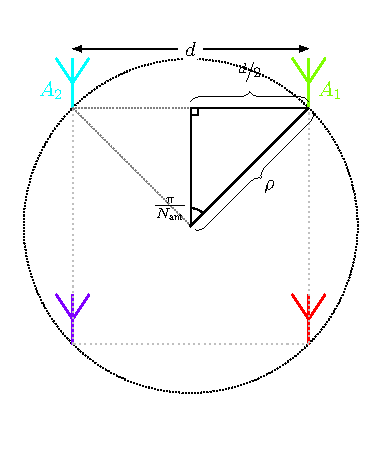
\includegraphics{../pictures/antennas_4.pdf}
        \label{fig:antennas:4}
    \end{subfigure}
    \hfill
    \begin{subfigure}[c]{0.525\textwidth}
        \centering
        \caption{$ \ac{Nant} = 5 $.}
        % % \resizebox{!}{0.7\textheight}{%
\begin{circuitikz}[american, voltage shift=0.5, line width=0.5,every node/.style={font = {\footnotesize\bfseries}}]

    \def\wavelength{8}
    \pgfmathsetmacro\d{0.5*\wavelength}

    \def\signalAngle{75}
    \def\antennaAngle{120}

    \def\closeRange{9}
    \def\farRange{\closeRange+13}

	\def\NAntennas{5}
	\pgfmathsetmacro\AngleAntennas{360/\NAntennas}
	\pgfmathsetmacro\ShiftAngleAntennas{-90+\AngleAntennas}

	\pgfmathsetmacro\RhoAntennas{\d/(2*sin(180/\NAntennas))}

    \def\centerarc(#1)(#2:#3:#4)% Syntax: [draw options] (center) (initial angle:final angle:radius)
    { ($(#1)+({#4*cos(#2)},{#4*sin(#2)})$) arc (#2:#3:#4) }

    \def\coordref[#1](#2){%

        \coordinate(sysref) at (#2);

        \draw[#1, -latex] (sysref) ++(-0.4,-0.3) -- ++(0.9,0) node[midway, below]{$x$};
        \draw[#1, -latex] (sysref) ++(-0.3,-0.4) -- ++(0,0.9) node[midway, left]{$y$};
        \draw[#1, -latex] \centerarc(sysref)(-90:180:0.25);
        \draw[#1] (sysref) node{$+$}
    }

    \coordinate (bottomleft) at (-4,-4);
    \coordinate (topright) at (4,4);


    % \draw[Red,dashed] (bottomleft) rectangle (topright);
    \clip (bottomleft) rectangle (topright);

    \coordinate (O) at (0,0);
    \coordinate (sourceAntenna) at (\signalAngle:\closeRange*\wavelength);
    % \draw [help lines, dashed] (bottomleft) grid (topright); % desenha grid
    % \draw [red] (O) node[draw,cross out] {}; % marca pont(0,0)

	\draw[densely dotted] (O) circle (\RhoAntennas);

    \draw[thick, cmyk_G] (O) ++(1*\AngleAntennas+\ShiftAngleAntennas:\RhoAntennas) node[dinantenna] (A1) {} node [above right] {$A_{1}$};
    \draw[thick, cmyk_B] (O) ++(2*\AngleAntennas+\ShiftAngleAntennas:\RhoAntennas) node[dinantenna] (A2) {} node [above left] {$A_{2}$};
    \draw[thick, cmyk_R] (O) ++(3*\AngleAntennas+\ShiftAngleAntennas:\RhoAntennas) node[dinantenna] (A3) {};
    \draw[thick, cmyk_C] (O) ++(4*\AngleAntennas+\ShiftAngleAntennas:\RhoAntennas) node[dinantenna] (A4) {};
    \draw[thick, cmyk_M] (O) ++(5*\AngleAntennas+\ShiftAngleAntennas:\RhoAntennas) node[dinantenna] (A5) {};

	\coordinate (A1_2) at ($(A1)!0.5!(A2)$);

	\draw[Black!25, dotted]
		(A1) --
		(A5) --
		(A4) --
		(A3) --
		(A2)
	;

	\draw[Black!50, densely dotted]
		(O) --
		(A2) --
		(A1_2)
	;

	\draw
		(A1) --
		(O) --
		(A1_2) --
		(A1)
	;

	\draw
         (A1_2)
           ++(0:0.125)
         --++(-90:0.125)
         --++(+180:0.125)
	;

	\node at (O) {\tiny\textbullet};

	\draw
		(O) ++(90:0.3) node[left, inner sep=1.5pt] {$\textstyle \frac{\pi}{N_\text{ant}}$}
		\centerarc(O)(1*\AngleAntennas+\ShiftAngleAntennas:90:0.3)
	;


    % Distânci d entre antenas
    \draw[latex-latex]
        ($(A1)+(0,1)$) -- ($(A2)+(0,1)$) node [midway, fill=white, circle, inner sep=1pt] {$d$}
    ;

    \draw[decorate, decoration={brace, amplitude=5pt}, thin]
    ($(A1)+({1*\AngleAntennas+\ShiftAngleAntennas-90}:0.1)$)
    -- coordinate (brace)
    ($(O)+({1*\AngleAntennas+\ShiftAngleAntennas-90}:0.1)$)
    ;

    \draw (brace) ++({1*\AngleAntennas+\ShiftAngleAntennas-90}:5pt)
        node[anchor=north west, circle, fill=white, inner sep=1pt] {$\rho$}
    ;

	\draw[decorate, decoration={brace, amplitude=5pt}, thin]
    ($(A1_2)+({90}:0.1)$)
    -- coordinate (brace)
    ($(A1)+({90}:0.1)$)
    ;

    \draw (brace) ++({90}:5pt)
        node[anchor=south, circle, inner sep=1pt] {$\sfrac{d}{2}$}
    ;

    % \coordref[Black!25](3.5,0);

\end{circuitikz}
% }


        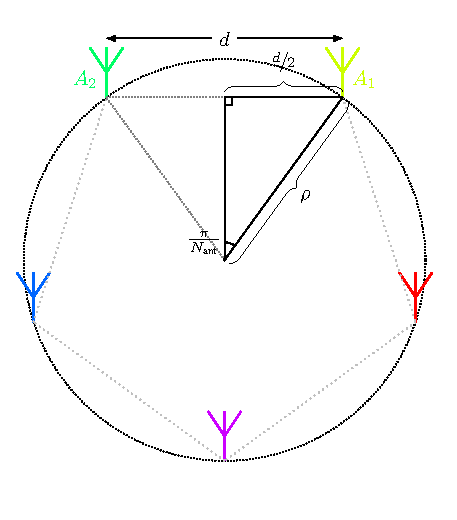
\includegraphics{../pictures/antennas_5.pdf}
        \label{fig:antennas:5}
    \end{subfigure}
    \hfill

    \caption*{Fonte: Autor.}
\end{figure}

A \autoref{eq:raio:poligono} descreve o raio \ac{rho} do círculo que circunscreve o polígono regular de \ac{Nant} antenas.
Este raio equivale à distância das antenas em relação ao ponto central do polígono.

\begin{equation} \label{eq:raio:poligono} % Diametro do circulo que circunscreve poligono de antenas
	\ac{rho} = \frac{\ac{d}}{2\cdot \sin\left(\displaystyle\frac{\pi}{\ac{Nant}}\right)}
\end{equation}

Cada antena é identificada por um índice \ac{k}, conforme a \autoref{eq:ant:idx}, e tem sua coordenada espacial definida como um valor complexo descrito na \autoref{eq:ant:coord}.
Essas coordenadas são definidas como números complexos para simplificar a análise do ângulo \textcolor{cmyk_M}{\ac{alphak}} em que um par de antenas \textcolor{cmyk_B}{\ac{Ak}} e $\textcolor{cmyk_R}{A_{k+1}}$ se dispõe em relação à geometria do sistema, conforme \autoref{eq:ant:angle}.

\begin{equation} \label{eq:ant:idx} % Indices das antenas
	\ac{k} = \left\{1, 2, \dotsc, \ac{Nant}\right\}
\end{equation}

% Coordenada da antena
\begin{equation} \label{eq:ant:coord}
	\textcolor{cmyk_B}{\ac{Ak}} =
    \ac{rho}
    \cdot \exp\left(\ac{imath}\cdot \ac{k} \cdot \frac{2\pi}{\ac{Nant}}\right) =
    \left( \operatorname{\mathcal{Re}}\left( \textcolor{cmyk_B}{\ac{Ak}} \right), ~\operatorname{\mathcal{Im}}\left( \textcolor{cmyk_B}{\ac{Ak}} \right) \right) =
    \left( \ac{xk}, ~ \ac{yk} \right)
\end{equation}

% Angulo do par de antenas
\begin{equation} \label{eq:ant:angle}
	\textcolor{cmyk_M}{\ac{alphak}} = \arg\left( \textcolor{cmyk_B}{\ac{Ak}} - \textcolor{cmyk_R}{A_{k+1}} \right)
\end{equation}

% {Calcular fase}

Para calcular a fase em uma antena, é interessante representar o sinal recebido como um valor complexo.
Uma forma de obter o complexo de fase consiste em analisar a correlação do sinal incidente \ac{w} com sinais de referência de mesma frequência que o sinal de interesse, em um período completo, \autoref{eq:periodo}.
Os valors \ac{Ik} (em fase) e \ac{Qk} (em quadratura) são calculados respectivamente pela correlação com um cosseno, conforme \autoref{eq:in_phase}, e com um seno, conforme \autoref{eq:out_of_phase}.
A \autoref{eq:Z} apresenta o valor complexo \textcolor{cmyk_B}{\ac{Zk}} de fase para a antena \textcolor{cmyk_B}{\ac{Ak}}.


% Periodo do sinal
\begin{equation} \label{eq:periodo}
    \ac{T} = \frac{2\pi}{\ac{omega}} = \frac{1}{\ac{f}}
\end{equation}

% In phase
\begin{equation} \label{eq:in_phase}
    \ac{Ik} =
    \int\limits_0^{\ac{T}} \cos\left(\ac{omega} \cdot\tau\right)
    \cdot \ac{w}\left( \ac{xk}, ~\ac{yk}, ~\tau \right) \partial \tau
\end{equation}

% Out of phase
\begin{equation} \label{eq:out_of_phase}
    \ac{Qk} =
    \int\limits_0^{\ac{T}} \sin\left(\ac{omega}\cdot\tau\right)
    \cdot \ac{w}\left( \ac{xk}, ~\ac{yk}, ~\tau \right) \partial \tau
\end{equation}

% Fase na antena
\begin{equation} \label{eq:Z}
    \textcolor{cmyk_B}{\ac{Zk}} =
    \frac{\ac{omega}}{\pi}\cdot\left(\ac{Ik} + \ac{imath} \ac{Qk}\right)
\end{equation}

% {Calcular defasagem entre antenas}

O cálculo de defasagem de sinal em um par de antenas consiste na análise de diferença de fase dos valores \textcolor{cmyk_B}{\ac{Zk}} e $\textcolor{cmyk_R}{Z_{k+1}}$ do par de antenas \textcolor{cmyk_B}{\ac{Ak}} e $\textcolor{cmyk_R}{A_{k+1}}$, conforme apresentado na \autoref{eq:dephase}.
Obtido o valor de defasagem \ac{DeltaPhi} entre o par de antenas, finalmente é possível calcular o ângulo \textcolor{Purple}{\ac{betak}} através da \autoref{eq:beta}, note que a simplificação somente é possível com valor de $\ac{d} = \sfrac{\ac{lambda}}{2}$.
A \autoref{fig:AoA:geometria} apresenta a geometria do sistema destacando os valores de interesse na análise de um dos pares de antenas, tomando $\ac{Nant} = 3$.

% Defasagem entre antenas
\begin{equation} \label{eq:dephase}
    \ac{DeltaPhi} =
    \textcolor{cmyk_B}{\ac{Phik}} - \textcolor{cmyk_R}{\Phi_{k+1}} =
    \arg\left(\textcolor{cmyk_B}{\ac{Zk}}\right) - \arg\left(\textcolor{cmyk_R}{Z_{k+1}}\right) =
    \arg\left(\textcolor{cmyk_B}{\ac{Zk}} \cdot \overline{\textcolor{cmyk_R}{Z_{k+1}}}\right)
\end{equation}

% Angulo do sinal em relação ao par de antenas
\begin{equation} \label{eq:beta}
    \textcolor{Purple}{\ac{betak}} = \arccos\left(\frac{\cancel{\ac{lambda}}}{\cancel{d}}\cdot\frac{\ac{DeltaPhi}}{\cancel{2}\pi}\right)
\end{equation}

\begin{figure}[htbp]
    \centering
    \caption{Geometria geral do sistema com $\ac{Nant} = 3$.}
    % \resizebox{!}{0.7\textheight}{%
\begin{circuitikz}[american, voltage shift=0.5, line width=0.5, every node/.style={font = {\footnotesize\bfseries}}]

    \def\wavelength{5}
    \pgfmathsetmacro\d{0.5*\wavelength}

    \def\signalAngle{75}
    \def\antennaAngle{120}

    \def\closeRange{9}
    \def\farRange{\closeRange+13}

	\def\NAntennas{3}
	\pgfmathsetmacro\AngleAntennas{360/\NAntennas}
	\def\ShiftAngleAntennas{-90}

	\pgfmathsetmacro\RhoAntennas{\d/(2*sin(180/\NAntennas))}

    \def\centerarc(#1)(#2:#3:#4)% Syntax: [draw options] (center) (initial angle:final angle:radius)
    { ($(#1)+({#4*cos(#2)},{#4*sin(#2)})$) arc (#2:#3:#4) }

    \def\coordref[#1](#2){%

        \coordinate(sysref) at (#2);

        \draw[#1, -latex] (sysref) ++(-0.4,-0.3) -- ++(0.9,0) node[midway, below]{$x$};
        \draw[#1, -latex] (sysref) ++(-0.3,-0.4) -- ++(0,0.9) node[midway, left]{$y$};
        \draw[#1, -latex] \centerarc(sysref)(-90:180:0.25);
        \draw[#1] (sysref) node{$+$}
    }

    \coordinate (bottomleft) at (-6,-0.5);
    \coordinate (topright) at (6,6.5);


    % \draw[Red,dashed] (bottomleft) rectangle (topright);
    \clip (bottomleft) rectangle (topright);

    \coordinate (O) at (0,0);
    \coordinate (sourceAntenna) at (\signalAngle:\closeRange*\wavelength);
    % \draw [help lines, dashed] (bottomleft) grid (topright); % desenha grid
    % \draw [red] (O) node[draw,cross out] {}; % marca pont(0,0)

    % Circulo de antenas
	\draw[densely dotted, opacity=0.25] (O) ++(90:\RhoAntennas) circle (\RhoAntennas);

    % Linhas do sinal de fundo
    \foreach \x [evaluate={\y=int((\x+\closeRange));\z=int((\x+\closeRange));}] in {-3,...,3} {
        \draw [black!75, very thin]
        (sourceAntenna) ++ (\signalAngle:-\z*\wavelength)
            % node[anchor=west, font = {\footnotesize\bfseries}]{$\y\lambda$}
        ($(sourceAntenna) + (\signalAngle:-\z*\wavelength) + ({10*cos(\signalAngle+90)},{10*sin(\signalAngle+90)})$)
            --
        ($(sourceAntenna) + (\signalAngle:-\z*\wavelength) - ({10*cos(\signalAngle+90)},{10*sin(\signalAngle+90)})$)
        % \draw [gray, thin] (sourceAntenna) circle (\z)
        ;
    }

    % Antenas
    \draw[thick, cmyk_R] (O) node[dinantenna] (A00) {} node [below] {$A_{k+1}$};
    \draw[thick, cmyk_G, opacity=0.75] (O) ++(60:\d) node[dinantenna] (A0d) {} node [below] {$A_{k+2}$};
    \draw[thick, cmyk_B] (O) ++(\antennaAngle:\d) node[dinantenna] (Ad0) {} node [above left] {$A_{k}$};

    \draw[very thin, Black!50] % Desenha eixo X
        (-0.5*\d,0) -- (2*\d,0) node[right] {$x$}
    ;

    % Ângulo alpha entre antenas
    \draw[thin, cmyk_M]
        (0.3,0) node [above right, inner sep=1pt] {\ac{alphak}}
        \centerarc(O)(0:\antennaAngle:0.3)
    ;

    % Comprimento de onda
    \draw[latex-latex]
        (A00) ++(\signalAngle+90:\wavelength) coordinate(signalAux)
         -- node [midway, fill=white, circle, inner sep=1pt] {$\lambda$} ++(\signalAngle:\wavelength)
    ;

    % Desenha senoide de fundo
    \draw[Goldenrod, domain=-8:8, samples=100] plot[shift={(signalAux)}, rotate=\signalAngle]({\x},{cos(\x * pi * 2 / \wavelength r)});

    % Direção do sinal
    \draw[very thick, dashed, -latex, Goldenrod]
        (A00) ++(1.5*\d,0) ++ (\signalAngle:-0.5*\d) -- coordinate(angleArrow) ++(\signalAngle:\d)
    ;
    % Angulo Theta do sinal
    \draw[thin]
        \centerarc(angleArrow)(0:\signalAngle:0.4) node [midway,above right,inner sep=1pt] {\ac{thetaAoA}}
    ;

    % Triangulo retângulo + quadradinho
    \draw[Black]

        (A00) --++($({\signalAngle-90}:{\d*sin(\signalAngle-\antennaAngle)})$) coordinate (pontoTriangulo) -- (Ad0) -- (A00)

        (pontoTriangulo)
          ++(\signalAngle:0.125)
        --++(\signalAngle-90:0.125)
        --++(\signalAngle+180:0.125)
    ;
    % Arco do angulo beta
    \draw[thin, Purple] \centerarc(Ad0)(180+\antennaAngle:180+\signalAngle:0.4)
        (Ad0) ++ (180+\signalAngle:0.5) node[below right, inner sep=1pt, fill=white, fill opacity=0.75,] {\ac{betak}}
    ;

    % Distânci d entre antenas
    \draw[latex-latex]
        ($(A00)+(0,1)$) -- ($(Ad0)+(0,1)$) node [midway, fill=white, circle, inner sep=1pt] {\ac{d}}
    ;

    \newcommand\CircleRadius{3cm}
    % special method of noting the position of a point
    \coordinate (P) at (50:\CircleRadius);

    \draw[decorate, decoration={brace, amplitude=5pt}, thin]
    ($(pontoTriangulo)+({\signalAngle+90}:0.1)$)
    -- coordinate (brace)
    ($(Ad0)+({\signalAngle+90}:0.1)$)
    ;

    \draw (brace) ++({\signalAngle+90}:5pt)
        node[anchor=east] {$\displaystyle\ac{lambda} \cdot \frac{\ac{DeltaPhi}}{2 \pi}$}
    ;

    \coordref[Black!25](3,3);

    % \foreach \x in {0,60,...,300} {
    %     \draw[thick] (\x:1 cm) -- (\x + 60:1 cm);

    %     \draw (\x + 30:1.732 cm) node[Gray, circ]{};
    %     \draw[Gray, dashed] (\x:1 cm) -- ++(\x: 0.9cm);
    %     \draw[Gray, dotted]
    %     %     % (\x:1 cm) arc (\x+240:\x+180:1cm)
    %         (\x:1 cm) arc [start angle=\x+120, delta angle=110, radius=1cm]
    %         (\x:1 cm) arc [start angle=\x+120, delta angle=-50, radius=1cm]
    %     ;
    % }

    % \draw (0,0) node [circ] {} node [below left,font={\scriptsize\bfseries}] {BS};
    % \draw[thick, densely dotted] (0,0) circle (1cm);

    % \draw[-latex] (0,0) -- (0:1cm) node[midway, below] {$R_c$};
    % \draw[-latex] (0,0) -- (90:0.866cm) node[midway, left] {$R$};

\end{circuitikz}
% }


    \label{fig:AoA:geometria}
    \caption*{Fonte: Autor.}
\end{figure}

Para cada par de antenas, são calculados dois valores \ac{thetak} conforme a \autoref{eq:theta:pmk}, equivalentes a dois valores possíveis para o \ac{thetaAoA}.
A \autoref{eq:theta:conj} define o conjunto \ac{Theta} dos valores aferidos de \ac{thetak} para todos os pares de antenas do sistema, este conjunto sempre terá $2 \cdot \ac{Nant}$ elementos, dos quais, metade estão próximos do real valor de \ac{thetaAoA} e os demais são valores distintos do objetivo e entre si.

% Conjunto de angulos calculados
\begin{equation} \label{eq:theta:pmk}
	\ac{thetak} = \textcolor{cmyk_M}{\ac{alphak}}\pm \textcolor{Purple}{\ac{betak}}
\end{equation}

% Conjunto de angulos calculados
\begin{equation} \label{eq:theta:conj}
	\ac{Theta} = \left\{\ac{thetak} ~\middle\vert~ \forall \ac{k}\right\}
\end{equation}

% {Escolha dos possíveis angulos}

Com os possíveis valores de \ac{thetaAoA} obtidos, é necessário estimar qual o valor correto.
Para isso, é criada uma lista auxiliar \ac{ThetaQuanti}, quantizando os valores de \ac{Theta} em intervalos de tamanho \ac{delta}, descrito na \autoref{eq:delta:range}.
A \autoref{eq:theta:quant} descreve a operação de quantização dos valores de \ac{Theta}, que, por se tratar de um cálculo auxiliar, utiliza-se o arredondamento para o inteiro mais próximo.
A quantização implica que os valores de \ac{Theta} serão agrupados por faixas de largura \ac{delta}.

% range_angle
\begin{equation} \label{eq:delta:range}
    \ac{delta} = \frac{\pi}{2 \cdot \left( 1 + \ac{Nant} \right)}
\end{equation}

% Angulos normalizados
\begin{equation} \label{eq:theta:quant}
    \ac{ThetaQuanti} =
    \left\{\left\lfloor\frac{\theta}{\ac{delta}}\right\rceil\cdot\ac{delta} ~\middle\vert~ \forall \theta \in \ac{Theta}  \right\}
\end{equation}

Salvo casos com muito ruído, espera-se que alguns valores em \ac{ThetaQuanti} se repitam, partindo disso, calcula-se \ac{thetaMo}, a moda estatística destes valores, conforme \autoref{eq:theta:moda}.
Esse valor deverá estar próximo ao \ac{thetaAoA}, e será utilizado na filtragem dos valores aferidos em \ac{Theta}.

% Moda entre angulos normalizados
\begin{equation} \label{eq:theta:moda}
    \ac{thetaMo} = \operatorname{\mathcal{M_o}}\left( \ac{ThetaQuanti}  \right)
\end{equation}

O conjunto \ac{ThetaFiltro} contém itens de \ac{Theta} que estejam ao redor do valor \ac{thetaMo} calculado, num intervalo de \ac{delta} para mais ou para menos, conforme \autoref{eq:theta:filtro}.


% Filtra no intervalo
\begin{equation} \label{eq:theta:filtro}
    \ac{ThetaFiltro} = \left\{\theta \in \ac{Theta}  ~\middle\vert~
    \ac{thetaMo} - \ac{delta} \leq \theta \leq \ac{thetaMo} + \ac{delta}\right\}
\end{equation}

Finalmente obtém-se o valor de \ac{thetaAoA} pela mediana dos valores em \ac{ThetaFiltro}, conforme \autoref{eq:theta:mediana}.

% Mediana
\begin{equation} \label{eq:theta:mediana}
    \ac{thetaAoA} = \widetilde{\ac{ThetaFiltro}}
\end{equation}




\section{Trabalhos relacionados}

Em seu trabalho, \citeauthor{horst2021localization} \cite{horst2021localization} analisa dois algoritmos de detecção de \ac{AoA}, realizando as análises em ambientes internos e utilizando matrizes de antenas.
O primeiro método analisado consiste em uma aproximação do ângulo, feita utilizando um \textit{software} fornecido pela Texas Instruments, fabricante do \textit{hardware} utilizado.
Já o segundo método, baseia-se na construção matemática do \ac{AoA} baseado na diferença de fase instantânea do sinal entre as antenas do sistema, uma abordagem semelhante à proposta neste trabalho.
Os resultados obtidos indicam que o método de aproximação teve melhor acurácia nos valores de ângulo.

A proposta de \citeauthor{zeaiter:hal-03693641} \cite{zeaiter:hal-03693641} busca validar a performance da detecção de \ac{AoA} em ambiente fechado, realizando a análise em diferentes modulações, larguras de canal e fatores de espalhamento.
Também propõe que, ao combinar de seu algoritmo de localização de \ac{AoA} com a função de autocorrelação, é possível analisar os dados de dois sinais recebidos simultaneamente.

Outro trabalho de \citeauthor{zeaiter:hal-03932846} \cite{zeaiter:hal-03932846} consiste um uma aproximação do \ac{AoA} utilizando um método de autocorrelação em um sinal \ac{LoRa} de baixa potência.
Seu objetivo consiste em detectar o sinal \ac{LoRa} operando em transmissão de baixa potência, caso onde a vida útil da bateria do sistema transmissor é estendida.
O algoritmo apresentado busca picos de autocorrelação no sinal recebido, além de utilizar \ac{FFT} para denotá-los e melhorar a \ac{SNR}.
Quando um pico é detectado, o algoritmo é capaz de encontrar o \ac{AoA}.

% O trabalho de \citeauthor{aernouts2020combining} \cite{aernouts2020combining} combina o método de filtro de partículas às medidas TDoA e \ac{AoA} obtidas em ambiente urbano denso.
% A performance é analisada de maneira comparativa à estimativa de TDoA e a um trabalho anterior baseado em combinação de matrizes.
% Seus resultados indicam um erro médio estimado de \SI{199}{\metre} sem o \ac{AoA}.

\citeauthor{bnilam20172d} \cite{bnilam20172d} propõe uma técnica que, sem qualquer informação prévia de largura de banda, consegue estimar \ac{AoA} do sinal recebido.
O sistema proposto consiste em uma \ac{UCA} seguida de um filtro transversal, também utiliza de vetores especiais de largura de banda variável junto com um estimador de relação sinal-ruído térmico para determinar simultaneamente \ac{AoA} e largura de banda do sinal recebido.

Em outro trabalho, \citeauthor{bnilam2017adaptive} \cite{bnilam2017adaptive} estudam a possibilidade de estimar \ac{AoA} para transceptores de \ac{IoT} em ambiente interno.
Também propõe um modelo probabilístico adaptativo que opera no modelo de estimativa de \ac{AoA}, incrementando sua performance.
Seus resultados indicam que estes métodos superam a performance de modelos probabilísticos estáticos tradicionais, tanto em acurácia de localização quanto em estabilidade no valor obtido.

Neste trabalho, \citeauthor{bnilam2019low} \cite{bnilam2019low} propõe um dispositivo de baixo custo capaz de estimar o \ac{AoA}, de forma que seja viável sua utilização em dispositivos de \ac{IoT}.
O dispositivo consiste numa conversão de vários \ac{SDR} individuais de baixo custo num único \ac{SDR} com múltiplos canais de \ac{RF}.
Seus resultados experimentais indicam que o dispositivo é capaz de estimar valores de \ac{AoA} de forma estável e acurada.

A proposta de \citeauthor{bnilam2020angle} \cite{bnilam2020angle} neste trabalho consiste em um novo algoritmo para determinação de \ac{AoA} chamado ANGLE (\textit{ANGular Location Estimation}), baseado em modelos probabilísticos para a resposta do sinal recebido.
Sua proposta ainda sugere duas versões do método, para o caso de amostragem única e de decomposição de subespaço, como utilizado no algoritmo MUSIC (\textit{MUltiple SIgnal Classification}).

\citeauthor{bnilam2020lora} \cite{bnilam2020lora} apresenta neste trabalho uma abordagem mais amigável para estimativa de \ac{AoA} em redes \ac{LoRa}.
O sistema proposto, denominado LoRay (\ac{LoRa} array) é composto por \textit{hardware} e \textit{software} preparados para fazer a estimativa de \ac{AoA} em ambiente urbano, onde o sistema foi validado.
O hardware utilizado foi descrito em um trabalho anterior \cite{bnilam2019low}.
Este sistema apresentou resultados estáveis e acurados para estimativa de \ac{AoA} tanto nos casos \ac{LoS} e quanto nos \ac{NLoS}.

% \citeauthor{steckel2018low} \cite{steckel2018low}

% \citeauthor{du2018long} \cite{du2018long}

Em seu trabalho, \citeauthor{niculescu2003ad} \cite{niculescu2003ad} propõe métodos para detecção de posição e orientação em cada nó de uma rede \textit{ad hoc}.
A proposta parte de possíveis problemas relacionados a utilização de \ac{GPS} em ambiente fechado

